\documentclass[a4paper, twoside]{report}

%% Language and font encodings
\usepackage[english]{babel}
\usepackage[utf8x]{inputenc}
\usepackage[T1]{fontenc}

%% Sets page size and margins
\usepackage[a4paper,top=3cm,bottom=2cm,left=3cm,right=3cm,marginparwidth=1.75cm]{geometry}

%% Useful packages
\usepackage{amsmath}
\usepackage{amssymb}
\usepackage{amsthm}
\usepackage{algorithm}
\usepackage{algpseudocode}
\usepackage{graphicx}
% \usepackage[capposition=top]{floatrow}
\usepackage{subfig}
\usepackage[numbers]{natbib}
\usepackage[colorinlistoftodos]{todonotes}
\usepackage[colorlinks=true, allcolors=blue]{hyperref}

% Shorthand commands
\newcommand{\R}{\mathbb{R}}
\newtheorem*{definition}{Definition}

\title{Evolutionary Algorithms for the Discovery of Cellular Automata Transition Functions}
\author{Manuj Mishra}

\begin{document}
\begin{titlepage}

\newcommand{\HRule}{\rule{\linewidth}{0.5mm}} % Defines a new command for the horizontal lines, change thickness here

%----------------------------------------------------------------------------------------
%	LOGO SECTION
%----------------------------------------------------------------------------------------


\includegraphics[width=8cm]{title/logo.eps}\\[1cm] % Include a department/university logo - this will require the graphicx package
 
%----------------------------------------------------------------------------------------

\center % Center everything on the page

%----------------------------------------------------------------------------------------
%	HEADING SECTIONS
%----------------------------------------------------------------------------------------

\textsc{\LARGE BEng Individual Project Interim Report}\\[1.5cm] % Name of your university/college
\textsc{\Large Imperial College London}\\[0.5cm] % Major heading such as course name
\textsc{\large Department of Computing}\\[0.5cm] % Minor heading such as course title

%----------------------------------------------------------------------------------------
%	TITLE SECTION
%----------------------------------------------------------------------------------------
\makeatletter
\HRule \\[0.4cm]
{ \huge \bfseries \@title}\\[0.4cm] % Title of your document
\HRule \\[1.5cm]
 
%----------------------------------------------------------------------------------------
%	AUTHOR SECTION
%----------------------------------------------------------------------------------------

\begin{minipage}{0.4\textwidth}
\begin{flushleft} \large
\emph{Author:}\\
\@author % Your name
\end{flushleft}
\end{minipage}
~
\begin{minipage}{0.4\textwidth}
\begin{flushright} \large
\emph{Supervisor:} \\
Prof. Andrew Davison \\[1.2em] % Supervisor's Name
\emph{Second Marker:} \\
TBC % second marker's name
\end{flushright}
\end{minipage}\\[2cm]
\makeatother

%----------------------------------------------------------------------------------------
%	DATE SECTION
%----------------------------------------------------------------------------------------

{\large \today}\\[2cm] % Date, change the \today to a set date if you want to be precise

\vfill % Fill the rest of the page with whitespace

\end{titlepage}

\begin{abstract}

Since the 1970s, John Conway's Game of Life, often shortened to just "Life", captured the imaginations of mathematicians, scientists and philosophers as an example of emergence, self-organization, and complexity arising out of simplicity. Since then, cellular automata (CA) have been used as models of physical\cite{wolf2004lattice}, chemical\cite{gray1983autocatalytic}, biological\cite{deutsch2021bio}, and social phenomena\cite{white2000high}. Recent work has used deep learning to learn CAs that converge to complex states (morphogenesis)\cite{mordvintsev2020growing} or recover a CA's transition function from a set of observations on its simulation (full rule dynamics)\cite{wulff1992learning}.\\

We investigate the use of evolutionary algorithms to this end. We build a cellular automaton simulator and evolutionary algorithm toolkit to address 3 learning objectives. The first is to induce desirable states in life-like CA, the discrete binary-state family of models in which Life belongs. In particular, we use life-like CA to build a procedural maze generator and learn transition functions that produce mazes with desirable qualities like long solution paths and numerous dead ends. The second objective is to learn the full rule dynamics of life-like CA. We show that genetic algorithms can quickly learn the full rule for 100\% of tested life-like CA from less than 10 observations, and usually from a single observation, albeit with longer training time. The third objective is to extend these results to Gray-Scott systems, the family of continuous state automata that simulate the reactions of two diffusive chemicals. These systems are discretizations of Turing's model for morphogenesis, a major theory in developmental biology. We extend the simulator to model continuous automata efficiently and extend the evolutionary algorithm toolkit to implement evolutionary strategies and a wider range of loss functions. In this case, we find that evolutionary algorithms struggle to learn full rule dynamics, instead converging to local optima.\\

This work extends existing work around procedural generation of mazes using cellular automata\cite{adams2017procedural} through improved learning processes, fitness functions, and post-processing algorithms. However, this is the first work to use evolutionary algorithms to learn the full rule dynamics of 2D cellular automata. In this regard, it sets a precedent for life-like CA, showing that all tested examples can be efficiently learnt with genetic algorithms. With optimizations to the learning procedure or additional computing power, future work could validate these results on larger test sets. Although this work is not able to learn full rule dynamics for Gray-Scott systems, future work can use the simulators and toolkit developed to test more advanced evolutionary computation techniques. The software developed in this project can also be used to conduct learning experiments on any variety of discrete or continuous CA systems.\\
\end{abstract}

\renewcommand{\abstractname}{Acknowledgements}
\begin{abstract}
[Acknowledgements here]
\end{abstract}

\tableofcontents
\listoffigures
\listoftables
\listofalgorithms


\chapter{Introduction}

\section{Motivation}

Predicting effects is easier than predicting causes. This is the statement of the Inverse Problem. In science, we find it easier to estimate observations from a parameterised model of the world than to deduce parameters from observations. This is a result of the causal opacity of time which eliminates information through the unforgiving forces of selection and entropy. Given knowledge of dinosaur evolution, we may have strong hope of predicting where fossils of certain species lie but to build a rigorous taxomony based on fossils alone is insurmountably harder. A physical model may allow us to predict the subatomic particles ejected when two protons collide at high speed but building physical theories based on these collisions is significantly more difficult, especially when there are multiple equally valid explanations. Regardless, the pursuit of the Inverse Problem is critical to advancing scientific theory around a system's behaviour. Observations can only validate or falsify but prediction paves the way for novel scientific models.\\

In this thesis, we tackle the inverse problem for cellular automata (CAs). These are simple yet powerful models of computation in which multiple "cells" on a discrete lattice are simultaneously updated at regular time steps. The state of each cell depends exclusively on the state of the cells in a local neighbourhood around it in the previous time step. This localised interaction makes CAs a useful abstract representation of physical and biological systems in the real world from gas molecule interactions[CITE] to human land behaviour[CITE]. Much like these systems, CAs can exhibit chaos, nonlinear dynamics, and the emergence of complexity. As well as simulatory models, CAs are powerful computational engines due to their inherently parallel structure. This makes their study a useful endeavour in the field of distributed computation too.\\

Top-down investigations into CA behaviour are vast and varied. Mathematical analyses seek to classify CAs and prove general results about long-term behaviour from intrisic properties. In the natural and social sciences, CAs are designed to model real world systems. Both of these endeavours seek to analyse the behaviour of a CA from its structure, transition function, and possibly initial conditions. In this thesis, we explore a bottom-up approach where we deduce the underlying properties of a CA by observing its behaviour. In particular, we utilise evolutionary algorithms to search across several classes of CA. Evolutionary algorithms (EAs) have long been held as effective tools for black-box optimisation problems. Grounded in the principles of Darwinian evolution, EAs traverse over a search space by performing selection, mutation, and crossover on a population of candidate solutions. Increasingly strong solutions are discovered as the fitness of the population grows. Using EAs, we tackle multiple optimisation problems from the imitation of particular CA behaviour to generation of desirable long-term states.\\

\section{Objectives}
We develop a system to discover cellular automata that are highly likely to exhibit a desired behaviour. Key aims include:
\begin{enumerate}
    \item \textbf{Learning Life-Like CA}\\
    Deduce the underlying transition rule behind cellular automata that exhibit chaotic and complex behaviour similar to that of Conway's Game of Life (see Subsection~\ref{sub:life}).
    \item 
\end{enumerate}

\section{Contributions}
The key contributions of this project are as follows:
\begin{enumerate}
    \item \textbf{Evolutionary Algorithm Toolkit}\\ A versatile toolkit that implements multiple evolutionary algorithms to train and optimise different classes of CA. We use this to successfully predict the update rule of binary outer-totalistic CA from observations of the CA running on random initial conditions. We show that this can be extended to continous automata by predicting the parameters of diffusion-reaction equations from simulations of chemical reactions.
    \item \textbf{Cellular Automaton Simulator}\\ A system that can efficiently simulate discrete and continuous cellular automata. This allows a broad range of fitness functions to be implemented in the EA toolkit. This can also render snapshots of the CA directly during simulation which allows animations to be efficiently generated afterwards.
    \item \textbf{Procedural Maze Generator}\\ A CA-based maze generation program that uses the EA toolkit to produce difficult mazes with characteristics optimised to user preference.
    
\end{enumerate}
\section{Technical Challenges}
\chapter{Preliminaries} \label{preliminaries}

\section{Cellular Automata}

A cellular automaton (CA) is a computational model that performs multiple parallel computations, each depending on local interactions, to produce complex global behaviour. We define a CA formally as follows.

\begin{definition}[Cellular Automaton]
A cellular automaton is an $n$-dimensional finite grid of computational units called cells. Each cell $c_i$ is characterised by:
\begin{itemize}
  \item A discrete state variable $\sigma_i(t) \in \Sigma$, where $i$ indicates the index of the cell in the lattice, $t$ indicates the current time step, and $\Sigma$ denotes the finite set of all state variables.
  \item A finite local neighbourhood set $\mathcal{N}(c_i)$ with cardinality $N$.
  \item A transition function $\phi:\Sigma^N \to \Sigma$ which takes local neighbour states as input. This is also known as the CA "update rule".
\end{itemize}

At each time step, the state of each cell is simultaneously updated according to the transition function. That is, $\sigma_i(t+1) = \phi( \:\{ \sigma_j(t) \: | \: c_j \in \mathcal{N}(c_i) \} \:)$
\end{definition}

Due to the breadth of systems studied in CA literature, the constraints of this definition are often altered to produce interesting arrangements. For example:
\begin{itemize}
  \item The structure need not be a square grid. CA have been studied on hexagonal grids\cite{encinas2007modelling}, aperiodic tessellations such as as the Penrose tiling\cite{goucher2012gliders}, and even randomly generated structures like the Voronoi partition\cite{shi2000development}.
  \item The system need not be deterministic. Probabilistic cellular automata (PCA) have stochastic transition functions which describe a probability distribution of possible outcomes for any given input. PCA are able to model random dynamical systems in the real world from stock markets\cite{bartolozzi2004stochastic} to infectious diseases\cite{mikler2005modeling}.
  \item The state space $\Sigma$ need not be finite. In this thesis we will explore multiple possible state variable representations including bit arrays and continuous vectors.
\end{itemize}
For the purpose of this thesis, we will assume the original definition of CA unless otherwise stated.

We consider a "neighbourhood function" for each cell $c_i \mapsto \mathcal{N}(c_i)$. This makes it easier to discuss neighbourhood sets of cells in the CA, each of which are typically homogenous. There are many possible neighbourhood functions for any given CA geometry. When defining the neighbourhood function, we select a distance metric $d:\mathbb{R}^n \times \mathbb{R}^n \to \mathbb{R}$ to measure the proximity of two cells and we set a threshold $T$ under which we consider two cells to be within each other's neighbourhood.
\[c_i \in \mathcal{N}(c_j) \iff d(c_i, c_j) \leq T\]

There are two neighbourhoods that are frequently used on Euclidean lattices. The \textit{von Neumann neighbourhood} contains all cells within a Manhattan distance of 1. For a 2D square lattice, this contains the cell itself and the 4 cells in the cardinal directions. For a 3D cubic lattice, it contains the central cell and a 6-cell octahedron around it. The \textit{Moore neighbourhood} contains all cells at a Chebyshev distance of 1. For a 2D square lattice, this is the central cell with the 8 neighbouring cells in a square around it. In the 3D case, it is a cube.

\begin{figure}[!h]
\centering
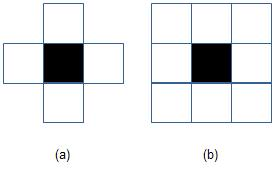
\includegraphics[width=.3\textwidth]{images/neighbourhoods.png}
\caption{(a) von Neumann Neighbourhood and (b) Moore neighbourhood on a 2D square lattice \cite{debasis2011survey}}
\label{fig:neighbourhoods}
\end{figure}

In a finite grid CA, border cells must be given special consideration since they do not have the same number of neighbours as interior cells and therefore cannot share the same neighbourhood function. One option is to define a case-wise neighbourhood function with different behaviour for border cells. Another option is to freeze the state of border cells. In the field of partial differential equations, this is known as setting "fixed boundary conditions".  The problem can also be circumvented entirely by relaxing the finite grid assumption and allowing cells to "wrap around" the grid. This is known as setting "periodic boundary conditions" and can be imagined visually as running the CA on an infinite periodic tiling or, alternatively, on a torus.\\


\subsection{Life-Like CA} \label{sub:life}
The most popular example of a CA is the Game of Life (henceforth "Life") formulated by John Conway in 1970 \cite{gardner1970fantastic}. It consists of a 2D grid of cells, each with a boolean state variable signifying that the cell is either "alive" or "dead". The transition rule takes as input the cell's own state $\sigma_i(t)$ and the number of living individuals in the cell's Moore neighbourhood (excluding itself), denoted $n_i(t)$. This is as follows:

\begin{equation}
  \phi(\sigma_i(t), n_i(t)) = 
\begin{cases}
  0 & \sigma_i(t) = 1 \text{ and } n_i(t) < 2 \text{  (Death by "exposure")}\\
  0 & \sigma_i(t) = 1 \text{ and } n_i(t) > 3 \text{  (Death by "overcrowding")}\\
  1 & \sigma_i(t) = 1 \text{ and } n_i(t) \in \{2,3\} \text{  (Survival)}\\
  1 & \sigma_i(t) = 0 \text{ and } n_i(t) = 3 \text{  (Resurrection)}\\
  0 & \text{otherwise}
\end{cases}
\end{equation}

Despite its simple setup and update rule, Life can exhibit the emergence of complex patterns. It is possible to simulate a fully universal Turing machine within Life\cite{rendell} and, as a corollary of the Halting Problem, this means that Life is undecidable. Given two arbitrary configurations, it is impossible to algorithmically determine whether one will follow the other.\\

Patterns found within Life include still lifes like the \textit{block} which are fixed-point solutions to the transition function as well as periodic oscillators like the \textit{beacon} which has period 2. There are also periodic patterns that move across the lattice such as the \textit{glider} pattern. It is possible to discover new stable patterns by repeatedly running specific rules on random initial patterns of a pre-determined density (called soups) and classifying the objects remaining after transient reactions have dissipated. Large-scale experiments of this nature are called "soup searches"\cite{flammenkamp}.\\

\begin{figure}[!h]
\centering
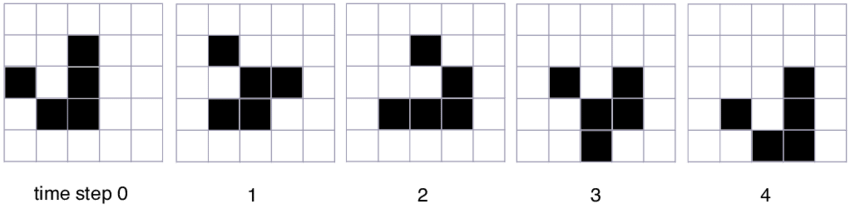
\includegraphics[width=0.8\textwidth]{images/life-glider.png}
\caption{The glider pattern in the Game of Life \cite{dorin2012framework}}
\label{fig:life-glider}
\end{figure}

A CA is considered "Life-like" if it exists on a 2D lattice, has binary state, uses the Moore neighbourhood function. Life-like cellular automata exist in two varieties: inner-totalistic and outer-totalistic.

\begin{definition}[Inner-Totalistic]
A Life-like CA is inner-totalistic if the output of the transition function depends only on the number of living cells in a cell's neighbourhood (including the cell itself).
\[
  \sigma_i(t+1) = \sigma_j(t+1) \iff \sum_{\mathclap{c_p \in \mathcal{N}(c_i)}}\sigma_p(t) = \sum_{\mathclap{c_q \in \mathcal{N}(c_j)}}\sigma_q(t)
\]
\label{def:inner-totalistic}
\end{definition}

\begin{definition}[Outer-Totalistic]
A Life-like CA is outer-totalistic if the output of the transition function depends on both the number of living cells in a cell's neighbourhood and the state of the cell itself.
\[
  \sigma_i(t+1) = \sigma_j(t+1) \iff \sum_{\mathclap{c_p \in \mathcal{N}(c_i)}}\sigma_p(t) = \sum_{\mathclap{c_q \in \mathcal{N}(c_j)}}\sigma_q(t) \quad \textnormal{and} \quad \sigma_i(t) = \sigma_j(t) 
\]
\label{def:outer-totalistic}
\end{definition}

As an example of the subtle difference here, consider the configurations shown in Figure~\ref{fig:two-moores}. An inner-totalistic CA would yield identical configurations in the next time step since both input configurations have 3 active cells in the neighbourhood set. However, an outer-totalistic CA would treat both configurations separately as one has an live centre cell and the other has a dead centre cell. This discrepancy corresponds to a great difference in the size of search spaces. There are $2^{10}=1024$ inner-totalistic CA but $2^{18} = 262144$ outer-totalistic CA. A B/S rulestring represents the transition function of an outer-totalistic CA in a form called birth-survival notation.\\

\begin{figure}[!h]
  \centering
  \hfill
  \subfloat{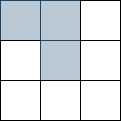
\includegraphics[width=.2\textwidth]{images/moore_1.png}}\hfill
  \subfloat{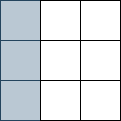
\includegraphics[width=.2\textwidth]{images/moore_2.png}}\hfill\hfill
  \caption{Two possible configurations of a Life-like CA}
  \label{fig:two-moores}
\end{figure}

\begin{definition}[Birth-Survival notation]
Let $N_b$ and $N_s$ be sets of integers. We say an outer-totalistic CA has rulestring \textnormal{B$N_b$/S$N_s$} if it has transition function:
\[
  \phi(\sigma_i(t), n_i(t)) = 
  \begin{cases}
    1 & \sigma_i(t) = 0 \text{ and } n_i(t) \in N_b \text{  (Birth)}\\
    1 & \sigma_i(t) = 1 \text{ and } n_i(t) \in N_s \text{  (Survival)}\\
    0 & \text{otherwise}
  \end{cases}
\]
\label{def:bs-notation}
\end{definition}

Using this notation, we can represent the Game of Life as B3/S23. In this thesis, when we refer to Life-like CA, we implicitly assume the outer-totalistic variety.

\subsection{Elementary CA} 
Elementary CA are defined on the simplest nontrivial lattice, a finite one-dimensional chain. The neighbourhood of each cell contains the cell itself and the two cells adjacent to it on either side. The state variable is a boolean which means there are $2^3 = 8$ possible neighbourhood state configurations. A transition rule maps each of these neighbourhood states to a resultant state and can therefore be represented as an 8-digit binary rule table $(t_7t_6t_5t_4t_3t_2t_1t_0)$ where configuration $(000)$ maps to $t_0$, $(001)$ maps to $t_1$, ..., and $(111)$ maps to $(t_7)$. Consequently, there are $2^8=256$ possible transition functions for elementary CA.\\

The Wolfram code, a number between 0 and 255 obtained by converting the binary rule table to decimal, is the standard naming convention for these rules. Rule 110 is particularly notable as it can exhibit class 4 behaviour \cite{wolfram2002} and is Turing complete \cite{cook2004universality}. Figure \ref{fig:rule-110} shows an example progression of a Rule 110 system. Each row of pixels represents the state of the automaton at one snapshot in time with the topmost row representing the randomized initial state. It shows the emergence, interaction, and subsequent dissipation of multiple long-lived impermanent patterns.

\begin{figure}[!h]
\centering
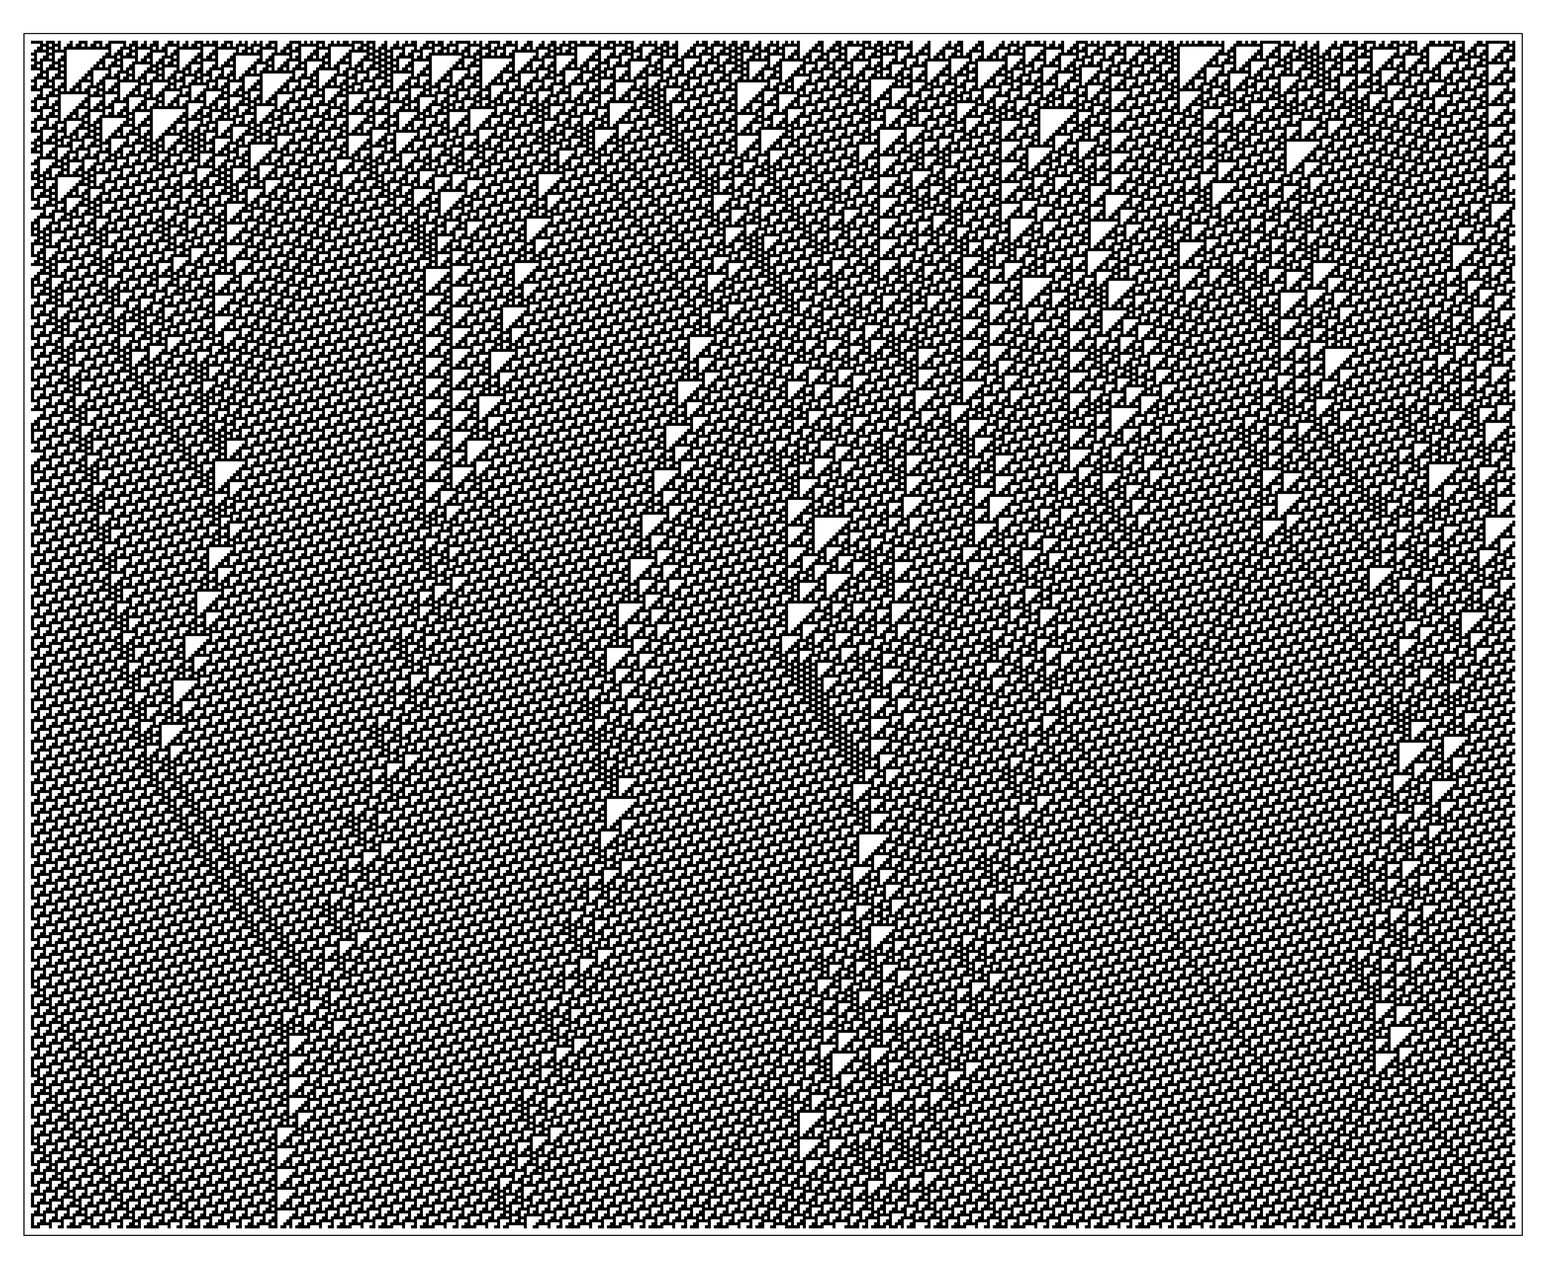
\includegraphics[width=0.7\textwidth]{images/rule-110.png}
\caption{Rule 110 progression with random initialisation \cite{wolfram2002}}
\label{fig:rule-110}
\end{figure}

\section{Turing Patterns}
Morphogenesis is the process by which a system develops into a particular shape or pattern.  Biologically, this is seen in most multicellular organisms which can robustly develop specialised organs and intricate skin patterns without any centralised decision-making. Through simple rules encoded in the genome and homeostatic feedback loops enforced through chemical signalling, a tissue knows exactly how to grow and when to stop.\\

In \textit{The Chemical Basis for Morphogenesis (Turing, 1952)\cite{turing1990chemical}}, Alan Turing proposes that spatially periodic phenomena in the natural world like the stripes on a zebra or the skin patterns on pufferfish can arise autonomously from random or uniform initial conditions through the interaction for two diffusible substances. These patterns are known as Turing patterns and Turing's model forms the basis of major theories in developmental biology. Such patterns are visible at all scales from the fold patterns of mammalian brains\cite{cartwright2002labyrinthine} to the distribution of matter in the Milky Way\cite{smolin1996galactic}.

\begin{figure}[!h]
\centering
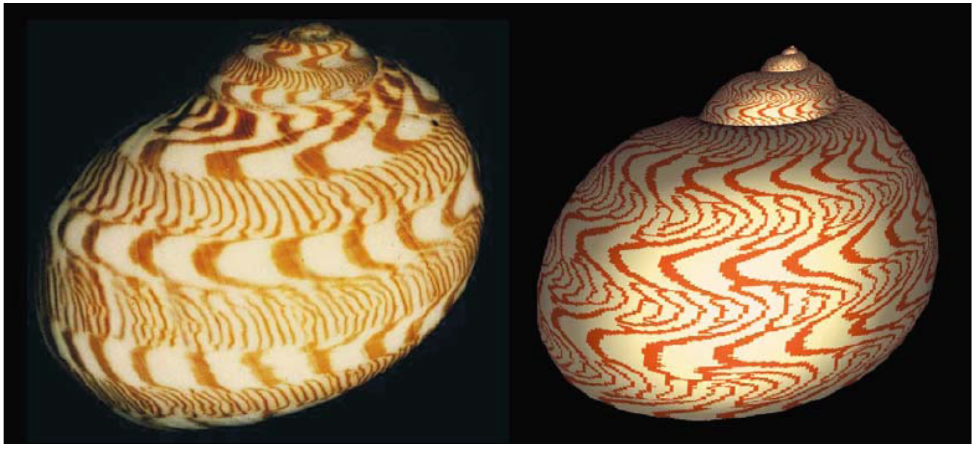
\includegraphics[width=0.6\textwidth]{images/turing-shell.png}
\caption{Complex patterns on sea shells(left) can be replicated using Turing patterns (right) \cite{meinhardt2009algorithmic}}
\label{fig:seashells}
\end{figure}

\subsection{Gray-Scott Model}

Turing patterns arise out of two component reaction-diffusion systems. One specific example is the Gray-Scott model\cite{gray1983autocatalytic} in which one component, $U$, is consumed while the other, $V$ is produced in a chemical reaction. In this thesis, we consider a simple reaction scheme called cubic autocatalysis where the following reaction occurs with a certain probability
\begin{equation}\label{eq:gs-main}
  U + 2V \rightarrow V
\end{equation}
To compensate for $U$ being consumed The system replenished $U$ and removes $V$ by rates controlled with feed and kill factors $f$ and $k$ respectively. The substances diffuse over the grid at rates $r_u$ and $r_v$. The system is characterised by two equations
\begin{definition}[Reaction-Diffusion System] \label{def:reaction-diffusion}
\begin{align} 
  \label{eq:gs-u} \pdv{u}{t} &= -uv^2 + f(1-u) + r_u \nabla^2 u\\
  \label{eq:gs-v} \pdv{v}{t} &= uv^2 - (f+k)v + r_v \nabla^2 v
\end{align}
\end{definition}
$u$ and $v$ represent the densities of each component in a given cell. $\dot{u}$ and $\dot{v}$ represent the change in these densities. Each density has three sources of change described by the three terms on the right hand side of each equation. The first term describes the reaction \ref{eq:gs-main} where 1 $U$ molecule reacts with 2 $V$ molecules which is why the term is a product of $u^1$ and $v^2$. The second term represents external inputs and outputs. In \ref{eq:gs-u}, the feed rate is multiplied by $1-u$ so that replenishment depends on current density. In \ref{eq:gs-v}, $v$ is multiplied by $-(F-k)$ so that $V$ is removed faster than $U$ is added. Finally, the third term describes the change in each density due to diffusion using the 2D Laplacian to get the difference between a cell's current state and the average of the neighbourhood cell states.\\

For most values of feed and kill rate, the Gray-Scott model attains one of two quiescent states, either completely dominated by $U$ or completely dominated $V$. However, there are certain feed and kill rates which elicit complex stable patterns. Many of these bear a strong resemblance to Turing patterns observed in nature.

\begin{figure}[!h]
\centering
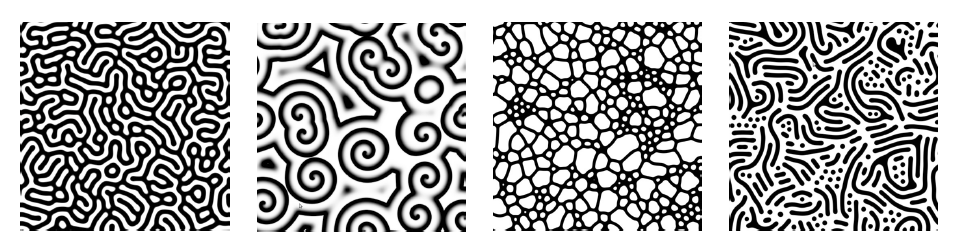
\includegraphics[width=\textwidth]{images/turing-patterns.png}
\caption{Turing patterns arising out of Grey-Scott model simulations\cite{sims}}
\label{fig:gs-turing-patterns}
\end{figure}

\section{Evolutionary Algorithms}

Evolutionary algorithms (EAs) are a family of heuristic-based search algorithms for black-box optimisation problems. They are inspired by biological evolution. A chromosome is an indirect encoding of a candidate solution. The structure of the chromosome is called the "genotype" and the behaviour of the corresponding candidate solution is called the "phenotype". The fitness of an individual is calculated from its phenotype. An evolutionary algorithm initializes population of chromosomes and modified them through repeated recombination, mutation, and selection. The purpose of recombination is to produce new solutions using "fit" attributes by combining aspects of existing candidates. Mutation, on the other hand, is applied to explore new areas of the search space by randomly perturbing existing candidates. Mutations may lead weaker candidates in the short term but is useful as a method of discovering new attributes that, over many generations, can produce fitter candidates. Finally, selection applies competitive pressure to the population, ensuring that the overall fitness of the population is improving and increasingly fit solutions are being discovered.\\

EAs are valued for their broad applicability as they require no information about the constraints or derivative of the objective function. In fact, an explicit representation of the objective function is not even neccessary to run an EA as long as candidates can be compared to each other. Selection pressure can then be introduced in the form of tournament-based elimination.\\

\subsection{Genetic Algorithms}

A genetic algorithm (GA) is a particular type of evolutionary algorithm with binary string genotype. For a genetic algorithm, we perform recombination by randomly picking two parents with replacement from the elite subset and mixing their chromosomes to produce a child. This is called crossover. We formalise the structure of a genetic algorithm as follows.\\

\begin{algorithm}
  \caption{Schematic Genetic Algorithm}\label{alg:ea}
  \begin{algorithmic}
  \Require $S$ - the set of possible chromosome values
  \Ensure $s^* \in S$
  \State $t \gets 0$
  \State $M_0 \gets \mu$ random individuals from $S$
  \While{stopping condition is false}
    \State \Call{Evaluate}{$M_t$}
    \State $P_t \gets$ \Call{SelectParents}{$M_t$}    \Comment{Parents}
    \State $\Lambda_t \gets$ \Call{Recombine}{$P_t$}  \Comment{Children}
    \State $Pmod_t \gets$ \Call{Mutate}{$P_t$}
    \State $\Lambda mod_t \gets$ \Call{Mutate}{$\Lambda_t$}
    \State $M_t+1 \gets$ \Call{SelectPopulation}{$Pmod_t$, $\Lambda mod_t$}
    \State $t \gets t+1$
  \EndWhile
  \State $s^* \gets$ \Call{FindBestCandidate}{$P_t$}
  \end{algorithmic}
\end{algorithm}

The initial selection phase ($\Call{SelectParents}$) uses a objective function, also known as a fitness function, to compare and select the top candidates. The latter selection phase ($\Call{SelectPopulation}$) produces a new population from the modified parents and children. Population-wide selection criteria can be enforced in this phase. For example, certain parents can be eliminated if they have survived for too many generations or, symmetrically, children can be granted immunity for a particular number of generations.\\

Genetic operators are the specific implementations of actions such as crossover and mutation. The most common mutation operator is pointwise mutation where each bit in the chromosome is flipped with some fixed probability $p$. The 3 common crossover operators used in genetic algorithms are
\begin{enumerate}
  \item Uniform Crossover: For each bit (or "gene") in the chromosome, copy the corresponding gene from one parent.
  \item Single Point Crossover: Randomly pick a split point. Take the all bits to the left of the split point from one parent and all bits to the right from the other.
  \item Multiple Point Crossover: Randomly pick $n$ split points. Alternate picking contiguous sections of the chromosome between split points from each parent.
\end{enumerate}

% \begin{figure}[!h]
% \centering
%     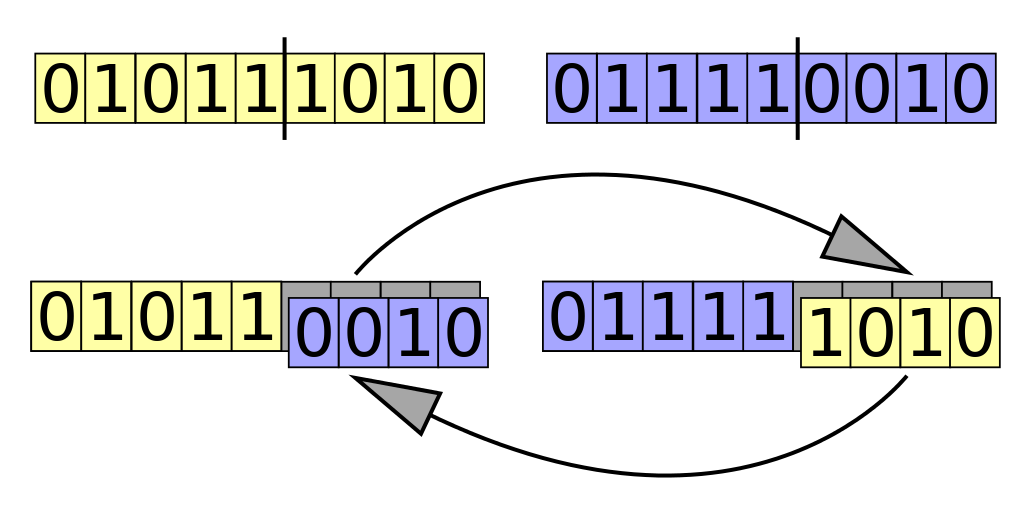
\includegraphics[width=.5\textwidth]{images/single-crossover.png}
%     \caption{Visualisation of single-point crossover on 9-bit chromosomes. \cite{singlecrossover}}
% \label{fig:single-crossover}
% \end{figure}


\chapter{Related Works}

\section{Learning Discrete CA with Genetic Algorithms}

\noindent
\textbf{Learning Algorithm for Modeling Complex Spatial Dynamics} (Meyer, Richards, and Packard, 1989) \cite{meyer1989learning} is a seminal work in this area. It creates a dynamical model from observations of discrete values evolving on a lattice over time. The model is represented as a binary probabilistic cellular automaton (PCA) whose neighbourhood set is learned by a genetic algorithm. The motivation for this work is to establish the form of CA which would most accurately describe patterns in the physical world directly from experimental data of physical interactions. In particular, Richards et al. \cite{richards1990extracting} builds on these techniques to find PCA rules that accurately predict the evolving patterns generated by the dendritic solidification of NH\textsubscript{4}BR.\\

Note that this goal is different from learning the entire transition function of a cellular automaton. This work merely aims to establish \textit{which} parameters in a local vicinity of the current state are most relevant to predicting the future state, not \textit{how} those parameters are combined and transformed to produce the future state.\\

The aim is to discover the most appropriate local neighbourhood set within a vicinity from the central cell that extends two steps in both space and time. This is the intersection of the Moore neighbourhood in time step $t-1$ and the von Neumann neighbourhood of range 2 in time step $t-2$. This comes to a 20 cell neighbourhood in space and time as visualised in Figure~\ref{fig:20-near}.

\begin{figure}[!h]
\centering
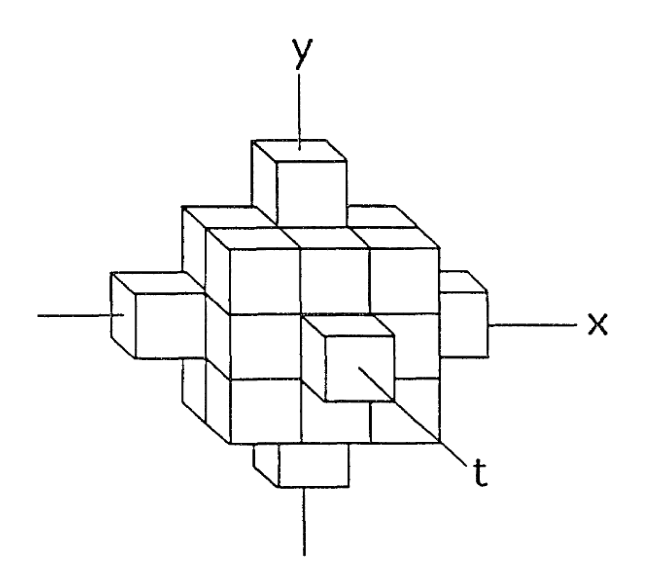
\includegraphics[width=0.3\textwidth]{images/20_neighbourhood.png}
\caption{20-cell, two step neighbourhood in space and time}
\label{fig:20-near}
\end{figure}

The full 20-cell neighbourhood is called the master template and each chromosome encodes some subtemplate ${s_1, ..., s_m}$. The fitness function used is
\begin{align*}
                    F &= I - \frac{2^m}{N}\\
    \text{where\:}  I &= \sum P(s, s_1,, ..., s_m)\log_2{\frac{P(s, s_1, ..., s_m)}{P(s)P(s_1, ..., s_m)}}
\end{align*}
Here, $I$ is the mutual information of the subtemplate and represents the amount of information (measured in Shannon bits) about the value of the central cell that can be obtained from the states of the cells in the subtemplate. It is calculated by summing across all $2^m$ configurations of the subtemplate in the data and across both values of $s \in \{0,1\}$. The second term in the fitness function ensures that subtemplates of varying sizes are treated appropriately by proportionately penalising large subtemplates that, by nature, will contain more information. In our case, $N=20$\\

The genetic algorithm initialises the population randomly. At each time step, a linear ranking of candidiates is performed and truncation selection is performed to pick the fittest subset. Crossover is applied between pairs of randomly selected candidates where the crossover point is an arbitrary cut in space-time on the master template. Point mutation is applied by either adding or removing a single cell from each candidate. This process is iterated to converge towards an optimum.\\

This method was successful at learning test data generated from a 1 time step Moore neighbourhood and data generated from 1 time step von Neumann neighbourhood with range 2. The algorithm successfully reproduces patterns generated by the first dataset precisely. However, unlike the first goal, the second goal neighbourhood is not subsumed by the master template. This means the algorithm can only hope to learn a similar template, not the exact objective. Despite this, the algorithm was able to find a neighbourhood set that produced correct behaviour 96\% of the time.\\

As the first notable exploration of learning CA properties with genetic algorithms, this paper devised a novel method for learning neighbourhood sets on binary PCA. It demonstrates the ability of this algorithm to predict neighbourhoods interior to the allocated search space as well as close approximations for objectives outside the search space.\\

This work raised many questions for future research. The most pertinent is whether it is possible to link learned rules to existing and future theoretical models. This work also only explored binary state CA but this excludes many continous variables relevant to data obtained from physical reactions such as the temperature field. An exploration of similar techniques on continous-state CA could be explored to closer approximate the partial differential equations that underlie the processes being explored.\\

Finally, this paper focused only on identifying the neighbourhood set of the CA that would closely approximate the interactions being studied. For the purposes of this thesis, we are interested in going beyond this and approximating the full transition function. In some cases we will fix the neighbourhood function used to reduce our search space under the assumption that further research could use techniques outlined in this paper to test whether better sub-neighbourhoods exist.
\chapter{Part I: Life-Like CA} \label{lifelike}

To learn life-like CA, we built an evolutionary algorithm toolkit. This is written entirely in Python making use only of basic data manipulation and scientific computing libraries such as NumPy, SciPy, and Pandas as well as media libraries like Matplotlib and Python Imaging Library.\\

\begin{figure}[!h]
\centering
    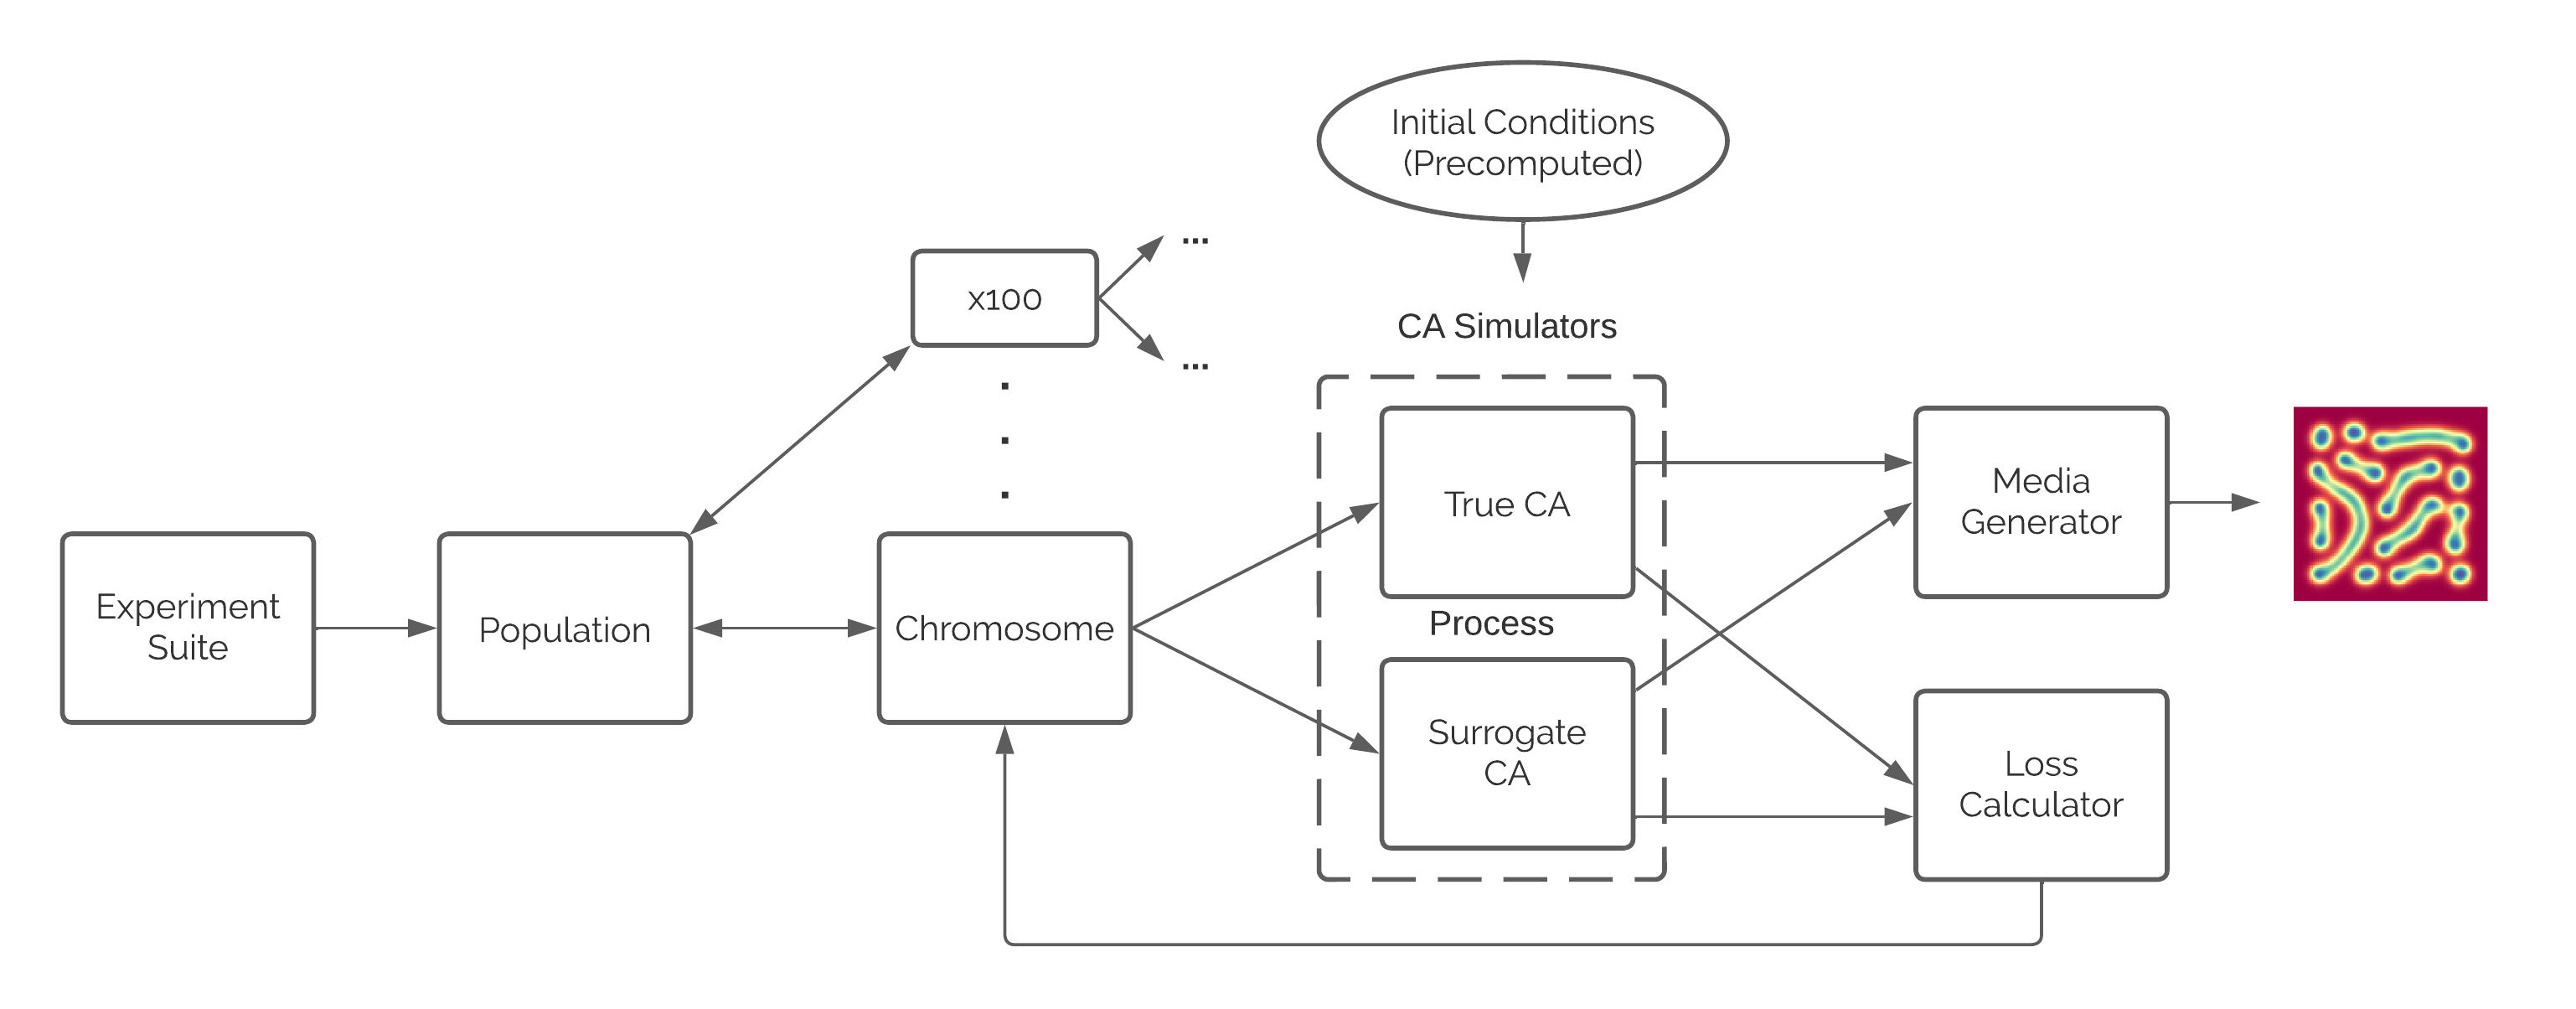
\includegraphics[width=\textwidth]{images/dataflow.png}
    \caption{Process for learning Life-Like and Gray-Scott CAs}
\label{fig:dataflow}
\end{figure}

It features the following key classes:
\begin{itemize}
    \item Experiment Suite: Includes methods and configurations for running evolutionary experiments.
    \item Population: Handles population-wide actions like crossover and elitism as well as tracking evaluation metrics like convergence and number of unique individuals seen.
    \item Chromosome: Handles individual actions like mutation, and fitness calculation.
    \item Simulator: Runs binary-state cellular automata and caches state data when needed
\end{itemize}

When learning a new class of CA or optimising for a new objective, an evolutionary algorithm is created by writing a new instance of the Population and Chromosome classes with implementations of the relevant evolutionary actions and objective function. An instance of the Simulator class must be created to implement the transition function from the parameters encoded in the chromosome. Experiments to test the algorithm can be shared across different objectives but the user may choose to write custom experiments depending on the goal at hand. Implementation of these experiments and their results are covered in detail in Section~\ref{sec:lifelike-evaluation}. We first explore the algorithms behind the learning process, the implementations of the Population, Chromosome, and Simulator classes, and delve into a practical application of the learning algorithm in the form of a maze generation program.

\section{Learning Process}

\subsection{Simulator} \label{subsec:simulator}
Due to the undecidability of various CA rules, the state of an automaton after a certain number of steps cannot, in general, be calculated without simulating each transition in turn. For this, a CA simulator was built.\\

The simulator stores the state of a 2D square CA of side length N in an NxN NumPy array. The CA is initialised with birth set B and survival set S which are given as direct arguments or calculated from the chromosome as shown in \ref{eq:bs-calc}. When simulating $n$ time steps, the simulator begins by caching the current state $X^{(t)}$. Then a neighbourhood matrix $M$ is calculated by convolving $X^{(t)}$ with kernel $\kappa$ where
\[
    \kappa = \begin{bmatrix}
        1 & 1 & 1\\
        1 & 0 & 1\\
        1 & 1 & 1
        \end{bmatrix}    
\]
Then, the value $M_{i,j}$ is the number of live neighbours of $X^{(t)}_{i,j}$. The convolution is calculated with wrapped boundaries to simulate periodic boundary conditions. The next state is calculated using the birth and survival sets as follows
\[
    X^{(t+1)}_{i,j}= (\lnot X^{(t)}_{i,j} \land n \in B) \lor (X^{(t)}_{i,j} \land n \in S)
\]
where the left conjunction corresponds to the case of a dead cell becoming alive and the right conjunction corresponds to a living cell surviving. If $X^{(t+1)} = X^{(t)}$, the cached state, then no further steps are calculated since a fixed point has been reached and $X^{(t + n)} = X^{(t + n - 1)} = ... = X^{(t)}$. Otherwise, the current state is cached and the simulator continues until n steps have elapsed or a fixed point is reached at some later stage. The simulator does not automatically detect periods of length greater than 1. The simulator allows the initial state $X^{(0)}$ to be set randomly with a particular density or set explicitly to a particular matrix. The latter is useful when simulating a surrogate CA which mimics the true CA and has to be updated regularly with known data. The simulator also allows the CA states to be saved at regular intervals as NumPy arrays and as images which are concatenated together into animated gifs.\\

\subsection{Genetic Algorithm} \label{subsec:life-like-ga}

A genetic algorithm (GA) is a particular type of evolutionary algorithm that acts on a population of indirect encodings called "chromosomes". The structure of the chromosome is called the "genotype" and the structure of the corresponding candidate solution is called the "phenotype". In this case, our genotype is a binary string encoding a transition function for a life-like CA. The corresponding phenotype is the behaviour of that CA over time. Genetic algorithms use actions called selection, mutation, and crossover to optimise the population and each of these is inspired by principles in biological evolution. We begin by formalising the structure of a genetic algorithm.\\

\begin{algorithm}
  \caption{Schematic Genetic Algorithm}\label{alg:ea}
  \begin{algorithmic}
  \Require $S$ - the set of possible chromosome values
  \Ensure $s^* \in S$
  \State $t \gets 0$
  \State $M_0 \gets \mu$ random individuals from $S$
  \While{stopping condition is false}
    \State \Call{Evaluate}{$M_t$}
    \State $P_t \gets$ \Call{SelectParents}{$M_t$}    \Comment{Parents}
    \State $\Lambda_t \gets$ \Call{Recombine}{$P_t$}  \Comment{Children}
    \State $Pmod_t \gets$ \Call{Mutate}{$P_t$}
    \State $\Lambda mod_t \gets$ \Call{Mutate}{$\Lambda_t$}
    \State $M_t+1 \gets$ \Call{SelectPopulation}{$Pmod_t$, $\Lambda mod_t$}
    \State $t \gets t+1$
  \EndWhile
  \State $s^* \gets$ \Call{FindBestCandidate}{$P_t$}
  \end{algorithmic}
\end{algorithm}

The initial selection phase ($\Call{SelectParents}$) uses a objective function, also known as a fitness function, to compare and select the top candidates. We seek to maximise fitness. Alternatively, selection may be based on minimising a loss function. Recombination produces a set of children that have similar properties to some subset of the parents. This exploits the cumulative generational knowledge in the parent candidates. Mutation explores new areas of the search space by perturbing properties of the parents and children. The latter selection phase ($\Call{SelectPopulation}$) produces a new population from the modified parents and children. Population-wide selection criteria can be enforced in this phase. For example, certain parents can be eliminated if they have survived for too many generations or, symmetrically, children can be granted immunity for a particular number of generations.\\

The optimization goal in this case is to find the transition rule that generated the observations made. A transition rule can be represented in a number of ways. Most intuitively, consider a birth and survival sets which dictates the number of neighbours that elicit a dead cell to become alive or a living cell to remain alive respectively. This can be encoded in a binary string which itself can be stored in integer form as shown in equation~\ref{eq:bs-calc}.

\begin{equation} \label{eq:bs-calc}
\begin{split}
    \text{Number of neighbours:}&\ 0\ 1\ 2\ 3\ 4\ 5\ 6\ 7\ 8\ |\ 0\ 1\ 2\ 3\ 4\ 5\ 6\ 7\ 8\\
    \text{Binary representation:}&\ 0\ 0\ 0\ 1\ 0\ 0\ 0\ 0\ 0\ |\ 0\ 0\ 1\ 1\ 0\ 0\ 0\ 0\ 0\\
    &\qquad\ \: \uparrow \qquad \qquad \qquad \ \: \: \uparrow \ \uparrow\\
    \text{Set representation:}&\quad \ \text{B:} \{3\} \qquad \qquad \ \ \: \text{S:}\{2, 3\}\\
    \text{Integer representation:}&\ \texttt{0b000100000001100000} = 16480
\end{split}   
\end{equation}

Each binary string chromosome has length 18, so the discrete search space is of size $2^{18} = 262144$. A population of $\mu$ chromosomes is chosen randomly from a distribution that is uniform over the density of the binary representations. As shown by [CITE], this is preferable to a distribution that is uniform over the integer representations since the density of the rule is more correlated with complexity properties than the integer value of the rule [EVIDENCE]. When initialising a random chromosome, a density $\rho$ is picked uniformly from $[0.0, 1.0]$. Then, each bit is a sample from the $\mathit{Bernoulli}(\rho)$ distribution.\\

At each iteration, the algorithm explores the search space through crossover and mutation, evaluates candidates through fitness calculations, and concentrates learned information through selection. In accordance with the $\frac{1}{5}$ rule [CITE], we produce $\lambda$ new children in each expansion stage and reduce down to $\mu$ elite candidates in each contraction stage with $\lambda \approx 4\mu$.Single-point crossover is used to produce new children. A crossover point c is picked between 1 and 17 and each of the parents is split at c. The left half of one parents chromosome is concatenated with the right half of the others chromosome. This process is repeated picking pairs of parents with replacement until enough children have been created.  Mutation is applied by flipping each bit in a chromosome with probability $\frac{1}{18}$ such that the expected number of bit flips per chromosome is 1. This is inspired by biological point mutation where individual base pairs in a biological genome are altered due to copying errors or environmental exposure. In reality, this is implemented more concisely by generating a mutation mask with expected density $\frac{1}{18}$ and applying XOR between the chromosome and mutation mask.\\

\begin{figure}[!h]
\centering
    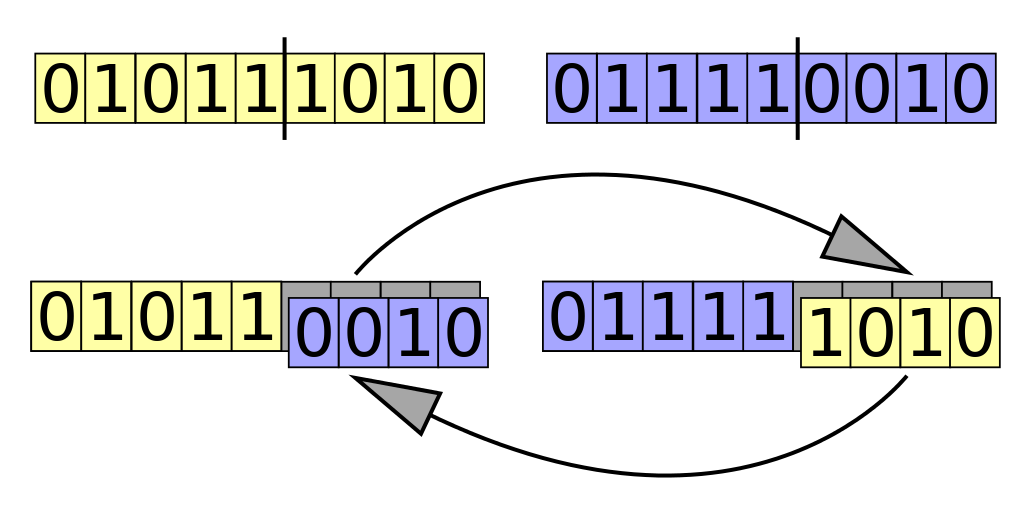
\includegraphics[width=.5\textwidth]{images/single-crossover.png}
    \caption{Visualisation of single-point crossover on 9-bit chromosomes. \cite{singlecrossover}}
\label{fig:single-crossover}
\end{figure}

When producing the next generation we consider selection criteria based on fitness and age. In a $(\mu + \lambda)$ selection setting, we produce a population of $\lambda$ children from $\mu$ parents and the next generation is selected from the collective. In a $(\mu, \lambda)$ setting, the next generation is selected exclusively from the $\lambda$ children. We can interpret this as an age restriction of 1 generation on the $\mu$ parent candidates. Common forms of selection include roulette and truncation. In truncation selection, all candidates are linearly ranked by fitness and the top $\mu$ candidates progress to the next generation. In roulette selection, the probability of each individual progressing to the next generation is proportional to its objective fitness.\\

\subsection{Fitness}

Fitness is calculated by running multiple CAs with the given transition function. For an $N \times N$ CA, it is infeasible to test on all $2^{N^2}$ initial conditions. Instead, a sample is picked. To ensure fairness, all CAs are tested on the same set of initial conditions sampled uniformly on densities between 0 and 1. In order to learn full rule dynamics, we design a fitness function that quantifies the ability of a candidate to convert the state observed in the goal CA at time $t$ to the state observed at time $t+\delta$ over $\delta$ time steps. Suppose $K$ observations of the goal CA are made producing states $X_{\delta_1}, X_{\delta_2} ..., X_{\delta_K}$ where the number of time steps between $X_{\delta_k}$ and $X_{\delta_{k+1}}$ is $\delta_{k+1}$. We define the loss of a candidate between observations $k$ and $k+1$ as the mean number of differing states between $X_{\delta_{k+1}}$ and the state of the candidate CA initialised at $X_{\delta_k}$ when observed $\delta_{k+1}$ time steps after initialisation. The loss between each observation is between 0 and 1. The fitness is defined by taking the mean of the losses and subtracting from 1.

\begin{definition}[Life-Like Fitness Function 1]
We define the fitness $F$ as
\begin{align*}
    F &= 1 - \bar{L}\\
    \textnormal{where\ } \bar{L} &= \frac{1}{N^2(K-1)}\sum_{k=1}^{K-1} X_{\delta_{k+1}} \oplus \phi^{\delta_{k+1}}(X_{\delta_k})
\end{align*}
where $\oplus$ is the XOR operator
\end{definition}

The number of observations and the values of the inter-observation times (or "step sizes") are hyperparameters. If $K$ is too high, we perform needless computations observing increasingly similar states as the CA stabilises. If $K$ is too low, we only observe early transient patterns instead of the long-lived patterns that characterise the objective rule. With regards to step sizes, we consider 3 possibilities.

\begin{enumerate}
    \item Constant: $\delta_1 = \delta_2 = ... = \delta_K = C$.
    \item Random Uniform: $\delta_k \sim \mathit{Uniform}(D_{min}, D_{max})$
    \item Random Increasing Uniform $\delta_k \sim \mathit{Uniform}(f_{min}(k), f_{max}(k))$
\end{enumerate}

where $f_{min}$ and $f_{max}$ are monotonically increasing functions of $k$. While a constant stepsize is simpler to implement, a random uniform stepsize is less likely to conflate periodic patterns in the CA with convergence. For example, consider \textit{Fumarole}, a 5-period oscillator in the Game of Life shown in Figure~\ref{fig:fumarole}. If $C=5$, the loss at each observation would be calculated using only one of its states. A rule that supports a still-life of the same configuration would be considered as optimal as the true rule. On the contrary, a random uniform stepsize with $D_{min} < 5 < D_{max}$ is extremely unlikely to land on the same state each time. The chances of this are only $\left(\sfrac{1}{(D_{max} - D_{min})}\right)^K$. Therefore, an algorithm with random uniform step size is much more likely to rank the true rule as fitter than the imposter. The random increasing uniform distribution goes a step further, increasing the expected value of $\delta_k$ as $k$ increases to allow time for late-stage patterns to appreciably change before making another observation.\\

\begin{figure}[!h]
\centering
            \subfloat{
\includegraphics[width=.15\textwidth]{images/fumarole/0.png}}\hfill
            \subfloat{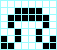
\includegraphics[width=.15\textwidth]{images/fumarole/1.png}}\hfill
            \subfloat{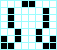
\includegraphics[width=.15\textwidth]{images/fumarole/2.png}}\hfill
            \subfloat{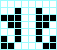
\includegraphics[width=.15\textwidth]{images/fumarole/3.png}}\hfill
            \subfloat{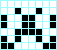
\includegraphics[width=.15\textwidth]{images/fumarole/4.png}}\hfill
            \caption{\textit{Fumarole}, a 5-period oscillator in the Game of Life. \cite{fumarole}}
\label{fig:fumarole}
\end{figure}

However, a fitness function that compares states cell-wise can be too fine-grained. It fails to capture macroscropic properties such as the density of live cells across different regions in the lattice. As a simple example, Figure~\ref{fig:singleres-fail} shows two predictions for a goal state. Prediction 1 clearly has a similar density and pattern to the goal but its live cells do not align with the live cells of the goal. Prediction 2 only has a single live cell making it quite different from the goal but due to the position of that cell, it achieves a much higher fitness than figure 1. To mitigate this affect, a multi-resolution fitness function is proposed which uses convolutions to capture density across broad regions.\\

\begin{definition}[Life-Like Fitness Function 2]
We define the multi-resolution fitness $F$ as
\begin{align*}
    F &= 1 - \bar{L}\\
    \textnormal{where\ } \bar{L} &= \frac{1}{N^2M(K-1)} \sum_{k=1}^{K-1} \sum_{m=1}^{M} \round{\omega_m \ast X_{\delta_{k+1}}} \oplus \round{\omega_m \ast \phi^{\delta_{k+1}}(X_{\delta_k})}\\
    \textnormal{where\ } \omega_m &= \frac{1}{m^2}
    \begin{pmatrix}
        1 & \ldots & 1\\
        \vdots & \ddots & \vdots\\
        1 & \ldots & 1\\
    \end{pmatrix}
    \in \mathbb{R}^{m \times m}
\end{align*}
where $\omega \ast f$ is a 2D convolution over image $f$ with filter kernel $\omega$ and $\round{.}$ is the integer rounding operator.
\end{definition}

The filter kernel used, $\omega_m$, is the all-ones matrix divided by the size of the kernel to ensure that $\omega_m \ast X$ has entries between 0 and 1 and that, after rounding, the convolution is a binary matrix with each cell representing whether there are more live or dead cells in an $m \times m$ region of the lattice. After XORing and summation, the loss $\bar{L}$ is between 0 and 1 and so is the fitness.

\begin{figure}[!h]
\centering
            \hfill
            \subfloat[Goal State]{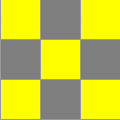
\includegraphics[width=.15\textwidth]{images/multires/1.png}}\hfill
            \subfloat[Prediction 1, fitness = 0]{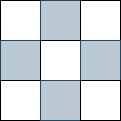
\includegraphics[width=.15\textwidth]{images/multires/2.png}}
            \hfill
            \subfloat[Prediction 2, fitness = 0.55]{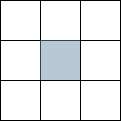
\includegraphics[width=.15\textwidth]{images/multires/3.png}}\hfill
            \hfill
            \caption{Example of fine-grain loss failing to capture macroscropic properties}
\label{fig:singleres-fail}
\end{figure}

\section{Maze Generation}

As a practical application of the genetic algorithm, we built a maze generation program. This uses a cellular automaton rule to randomly generate a unique maze-like structure which is modified to ensure a solution path exists. A genetic algorithm, based on the one designed in subsection~\ref{subsec:life-like-ga} is used to find the chromosome that tends to produce the "best" maze according to a user-inputted definition of "best" using quantitative factors such as length of solution and number of dead ends. The maze is made up of cells in one of two states. The "live" or 1 state represents walls and the "dead" or 0 state represents possible path cells. There are also two special states which represent the start and goal cell.\\

This has some similarities to a work by C. Adams\cite{adams2018evolving} which also looks at the application of CAs in maze generation. However, this application differs notably from Adams' in both the evolution algorithm and fitness function design. Key features in our maze generator include the notion of failed rules, the stochastic region merging algorithm, and automated loss calculation (i.e. no external human input required to rank mazes).

\subsection{Procedural Generation}
A maze is generated from a chromosome in three stages: growth, region search, and region merging. During the growth stage a CA is run for a fixed number of iterations, typically 50, using the birth and survival sets encoded in the chromosome. This process is explained in detail in \ref{subsec:simulator}. The region search stage uses iterated breadth first searches to find all disconnected regions within the maze. The region merge stage connects these regions randomly until a connected path exists from the start cell to the goal cell. In order to perform the merge stage, two data structures are populated during the find stage. The first is a hashmap from each cell to the region number of the region it occupies. The second is the reverse, a hashmap from each region number to the set of cells in that region.

\begin{algorithm}
  \caption{Region Finding Algorithm}\label{alg:region-find}
  \begin{algorithmic}
  \Require $X$ - the state of the CA after the growth stage
  \Ensure cells[($c_x$, $c_y$)] = $r_c \iff$ ($c_x$, $c_y$) $\in$ regions[$r_c$]

  \Comment{Initialisation}
  \State cells $\gets$ empty dictionary of type \{(int, int): int\}
  \State regions $\gets$ empty dictionary of type \{int: set\{int\}\}
  \State spaces $\gets$ set of cells in X with state 0

  \Comment{Find first region}
  \State $r_1 \gets$ \Call{BFS}{start-cell, $X$}
  \State \Call{UpdateDicts}{$r_1$, 1}
  
  
  \Comment{Find remaining regions}
  \State counter $\gets 1$
  \While{spaces not empty}
    \State counter $\gets$ counter + 1
    \State startCell $\gets$ randomly chosen 0-state cell
    \State $r \gets$ \Call{BFS}{startCell, $X$}
    \State \Call{UpdateDicts}{$r$, counter}
  \EndWhile

  \Comment{Update Function}
  \Procedure{UpdateDicts}{region, index}
    \For{$c$ in region}
        \State cells[$c$] = index
        \State regions[index].add($c$)
    \EndFor
    \State spaces $\gets$ spaces - $r$
  \EndProcedure
  \end{algorithmic}
\end{algorithm}

It is crucial for the region merging algorithm to be stochastic. If it is deterministic and merges regions according to a pre-designed pattern, the genetic algorithm is incentivised to learn rules that lend themselves well to this pattern. For example, if mazes will longer solution paths are considered fitter and the merging algorithm connects regions in horizontal bands sweeping left-to-right (as in \cite{adams2018evolving}) then the evolutionary process is incentivised to produce rules with shorter horizontal corridors over longer vertical corridors. This is in direct conflict with the fitness function. To avoid this, we design a stochastic region merging algorithm. It begins with the region containing the start cell. Each wall cell bordering this region is examined to determine whether removing the cell would connect to a distinct region. One of these wall cells is randomly chosen and removed. This process repeats on the union of the two joined regions. If no such wall cells exist, the simulation is deemed unsuccessful. If a chromosome does not yield a minimum percentage of successful simulations, it is assigned a fitness of 0 and usually removed from the population in the following iteration.\\


\begin{algorithm}
  \caption{Region Merging Algorithm}\label{alg:region-merge}
  \begin{algorithmic}
  \Require cells, regions, X
%   \Ensure cells[($c_x$, $c_y$)] = $r_c \iff$ ($c_x$, $c_y$) $\in$ regions[$r_c$]
  \State visited $\gets$ regions[1]
  \While{True}
    \State fringe $\gets$ \Call{OneNeighbours}{visited}
    \If{goalCell in fringe}
        \State return True \Comment{Success}
    \EndIf
    \State candidates $\gets$ []
    \For{$f$ in fringe}
        \State zeros $\gets$ \Call{ZeroNeighbours}{$f$}
        \If{length(zeros - visited) > 0}
            \State candidates.append($f$)
        \EndIf
    \EndFor
    \If{length(candidates) > 0}
        \State $c \gets$ \Call{PopRandom}{candidates}
        \State visited.add($c$)
        \State X[$c$] = 0
        \State newRegions $\gets$ \{cells[$d$] for $d \in$ \Call{ZeroNeighbours}{$c$}\}
        \State visited $\gets$ visited $\cup$ \{regions[$r$] for $r \in$ newRegions\}
    \Else
        \State return False \Comment{Failure}
    \EndIf
  \EndWhile
  \State
  \State where \Call{OneNeighbours}{} and \Call{ZeroNeighbours}{} return the 1-state and 0-state neighbours of a cell respectively.
  \end{algorithmic}
\end{algorithm}


\subsection{Genetic Algorithm}

The algorithm, as before, initialises a random population of chromosomes and evolves them using bitwise mutation, single-point crossover, and $(\mu + \lambda)$ truncation selection. The aim of the fitness function is to assess the maze using quantitative metrics that can be calculated in a computationally efficient way. For example, the number of vacant cells reachable from the start cell is an important metric because, if this is too low, a large portion of the maze is wasted space. It can also easily be computed by performing a breadth first search in the region containing the start cell and recording the number of vacant cells in the maze that exist outside this region. This calculation takes linear time with respect to the number of cells in the automta. In the final algorithm, two metrics are used: the number of dead ends and the solution path length. These factors work well as they oppose each other. A maze with a long solution tends to have long corridors whereas a maze with many dead ends tends to have shorter corridors and more decisions to make at each junction. Assuming a maze with at least one solution, both metrics can be calculated simultaneously in a single breadth-first search traversal. A cell is considered to be a dead end if all its neighbours are wall cells or vacant cells that have already been visited.\\

Initially, the fitness function $f(c_i) = s + \lambda d$ where s is the solution path length and d is the number of dead ends, was considered. 
[EXPAND HERE]
However, this is not normalized as the solution length and number of dead ends are not on the same scale. Furthermore, we cannot normalize each metric individually based on the range of values present in a given generation since the ranges vary from experiment to experiment and generation to generation. Instead, a truncated linear selection is performed where each chromosome is ranked separately by each metric and the fitness function is defined as $f(c_i) = r_s + \lambda r_d$ where $r_s$ and $r_d$ are the rank of the cell in the population according to solution length and number of dead ends respectively. The top $\mu$ candidates by fitness are picked.

\section{Software Engineering Design}

In this chapter, we summarise key software engineering design decisions when writing the evolutionary algorithm toolkit.

\subsection{Media Generation}
To extract insights from the toolkit, metrics and media must be generated. The experiment suite class configures populations according to user-defined parameters and records metrics from the population at each epoch in Pandas dataframes. These metrics are saved to a csv file at regular intervals. Media is generated automatically once an experiment has finished. The top 3 solutions are simulated again. At regular intervals, a media save is triggered whereby the state of the running automaton is converted into a 2D regular raster graphic using Matplotlib and saved as a png file in a temporary folder. If there are multiple stages of simulation (e.g. growth, region find, and region merge), one temporary folder is created per stage. After simulation, these images are stitched together into gif animations using the Python Imaging Library (PIL). The final state is also saved as a png image and in its original array form as a npy file. The temporary frame files are deleted. Analysis and visualisation of population-wide properties is done manually after the experiments have completed.\\

\subsection{Chromosome Class}
One notable point is about the initialisation and update of the Chromosome class. To avoid repeated calculations converting between birth/survival sets and binary rule strings, the Chromosome class must keep track of the binary form and sets form of the rule simultaneously. Although Python usually allows direct access to private class fields, it is verbose and error-prone to update all other fields every time a single field needs to updated. We use \texttt{@property} decorators to automatically enforce synchronisation between these fields by defining an implicit setter function that updates the birth and survival sets every time the binary rule string is updated.\\

The two initialisation methods for chromosomes based on sampling uniformly across density and sampling uniformly across value are implemented using the factory method design pattern. \texttt{Chromosome.random\_density()} and \texttt{Chromosome.random\_value()} are public factory methods that generate a binary rule string and call an internal factory method \texttt{Chromosome.from\_rstring()} which calculates the birth and survival sets then passes all three parameters to the constructor which creates a new \texttt{Chromosome} object.

\section{Evaluation} \label{sec:lifelike-evaluation}

\subsection{Diversity}
When looking to quantify
\chapter{Maze Generation}

\section{Region Merging Algorithm}

\section{Fitness Evaluation}

\section{Selection and Quality-Diversity}


\chapter{Gray-Scott Models}

\section{Evolutionary Strategy}
\chapter{Project Plan}

This project is based on improving and building upon very recent work in a relatively new line of exploration.
As such, much of the work is experimental.
This project demands a level of familiarity with the relevant theory, methods, and technologies around CA and machine learning which is developed in the early stages.
The middle stages begin by reproducing existing results from recent work on CA morphogenesis and regeneration. This includes new research into morphogenesis for graph CA. 
Following this, the key goal is to developing theoretical ideas to improve the methods used to produce these results. These could be more efficient versions of existing ideas, extrapolating ideas from one domain to another (e.g. applying pattern-damage training methods from Mordvintsev et al \cite{mordvintsev2020growing} to the context of graph CA introduced by Grattarola et al. \cite{grattarola2021learning}), or even entirely novel ideas.
Finally, the project aims to test and improve the efficacy of these methods through experimentation and iteration. 
At this stage, extension goals could also be addressed. 
These include practical work like producing rich demonstrations to allow layman audiences to interact with the research. 
They could also include theoretical work like investigating the connection between periodic and fixed-point solutions in CA rule space and devising a way to incentivise a system to converge to a fixed point solution over a periodic one.
Each of these 3 stages is expected to take a roughly equal amount of time.
Throughout each of the stages, the project write-up will continue to develop.
The interim report will be written during the latter half of stage 1 and the earlier half of stage 2.
This will provide a strong basis for the final report which will be written in the latter half of stage 2 and the earlier half of stage 3.

\section{Key Milestones}
The key milestones in this project along with the projected dates of completion are outlined as follows.\\

\textbf{Nov / Dec 2021}: The first milestone is to decide on specific aims for the project. 
This was achieved by the planned deadline. 
The goals for this project came naturally out of an exploration into the literature around morphogenesis in cellular automata.
Since CA are a relatively mature concept, there is a large body of research in this area.
However, the background reading for this project focused on a subset of this body, concerning the applications of machine learning to learn transition rules.
Since the seminal paper by Wulff and Hertz in 1992 \cite{wulff1992learning}, this was a relatively stagnant area of research until the breakthrough work by Mordvintsev et al in 2020 \cite{mordvintsev2020growing}.
This opened up many possible areas of exploration including self-classifying CAs \cite{randazzo2020self-classifying}, adversarial attacks on morphogenetic CAs \cite{randazzo2021adversarial}, and learning graph CA \cite{grattarola2021learning}.\\

\textbf{Jan / Feb 2022}: Following this, the next goal is to write an interim report which introduces the topic, lays out preliminary knowledge, discusses related work, and details a plan for project execution and evaluation.
It also lays a strong basis for the final project report.
This goal was also achieved on time.
The next technical milestone is to replicate the procedure outlined in the Learning Graph Cellular Automata paper \cite{grattarola2021learning} and reproduce the results on the 5 example point clouds.
It also involves experimenting on new point clouds, eliciting both periodic and fixed-point behaviour.
This will allow me to deeply familiarise myself with the methods used in this paper and gain an intuition for ways in which they could be improved.\\

\textbf{Mar / Apr 2022}: The next milestone would be to devise appropriate machine learning models to train a GCA to perform morphogenesis on point clouds that are smaller in number than the target. 
This will involve going beyond current research on GCA to develop a better understanding of shape and structure. 
For example, the GCA will need to understand what it means for two point clouds of differing density to both be in "the shape of a bunny". 
This will require a more complex metric than the simple Euclidean distance between training points and target points that was used when training and testing on point clouds of equal density.
This training method should then be adapted to induce regenerative behaviour in solutions.
One promising avenue of exploration here would be the damage-based training techniques seen in Growing Cellular Automata \cite{mordvintsev2020growing}.\\

\textbf{May / Jun 2022}: At this point, the goals for the final two months of this project are flexible. If the project is progressing slower than planned, then these months provide a good opportunity to catch up. In the event of a pivot, these months also provide some safety buffer to expand the scope of the project in a different direction from a fall-back position. For example, if the damage-based training proves to be inadequate at producing regenerating solutions in the graph context, then exploring new techniques from different areas of research and developing new ideas will require some additional time that these months can provide.
However, if the project is progressing well, then these months will be used to engage with extension goals.
One extension goal is to produce explorable explanations of the research.
This will involve rewriting some of the machine learning models in Tensorflow.js and producing interactive web demonstrations in a style similar to that used by the Distill journal \cite{distill}.
Another extension goal is to explore the theory behind different types of class 2 CAs.
This is of particular interest as it is useful to seperate fixed-point solutions from periodic solutions and understand the difference between them.
The ideal scenario here would be to devise a method of incentivising machine learning systems to converge to fixed-point solutions over periodic solutions.
Although the final report will continue to develop throughout the whole project, a substantial portion of the last month will also be dedicated towards improving and polishing the final report.
    
\chapter{Conclusions}

\section{Further Work}

\subsection{Procedural Generation}

\subsection{New CA Topologies}

\subsection{Evolutionary Strategies}

\subsection{Neural Networks}

\todo{Add appendix w/ BFS on grid algorithm}

\chapter{Evaluation} \label{evaluation}

\section{Metrics}
Alongside properties discussed in Sections \ref{sec: life-like-exploration} and \ref{sec: gs-exploration}, we design metrics to categorise CA and assess the effectiveness of evolutionary algorithms.

\subsection{Dynamic Metrics}
We say a dynamic metric is one that tells us about the way a CA's state changes over time. Two useful dynamic metrics are periodicity and volatility.

It is useful to know when a CA has converged to a fixed point or periodic solution. By estimating the portion of initial conditions that enter a periodic state, and the speed with which they do so, we can infer the Wolfram class of CAs with reasonable accuracy. The key distinction we intend to make here is between CAs in class 1 or 2 against CAs in class 3 or 4. The former two classes should converge relatively quickly for almost all ICs whereas the latter two will not converge for a significant proportion of ICs.

\begin{definition}[CA convergence to a periodic state]
 If a state previously visited at time step $t$ is produced again at step $t+\delta$, the rule is said to have converged to a periodic solution at $t+\delta$ time steps with period $\delta$. If $\delta = 1$, this is called a fixed point solution. 
\end{definition}

For the trivial initial conditions with all zero-cells or all one-cells, all life-like CAs will converge to a periodic state with $\delta \leq 2$. The proof of this is detailed in \ref{quiescent-nullity}.

\begin{definition}[Quiescence]
A CA is quiescent if all cells are in the same state. A CA with each cell $c_i$ in state $\sigma_i(t) = 0$ is denoted $\vec{0}$ and the opposite quiescent CA with $\sigma_i(t) = 1$ is denoted $\vec{1}$. 
\end{definition}

\begin{lemma}
A quiescent life-like CA is at a fixed point or oscillates with period 2.   
\end{lemma}

\begin{proof} \label{quiescent-nullity}
Consider an arbitrary cell $c_i$ in $\vec{0}$. $\sigma_i(t)$ is the state of $c_i$ at time t and $n_i(t)$ is the number of live cells in the neighbourhood of $c_i$ not including itself. Initial conditions are $\sigma_i(0) = 0 \text{\ and\ } n_i(0) = 0$.
\begin{multicols}{2}
\noindent If $0 \notin B$:\\
\null \quad $\sigma_i(1) = 0 \text{\ and\ } n_i(1) = 0 $\\
\null \quad $\implies$ convergence to $\vec{0}$ with period 1.\\
\columnbreak\linebreak
\noindent If $0 \in B$:\\
\null \quad $\sigma_i(1) = 1 \text{\ and\ } n_i(1) = 8 $\\
\null \quad If $8 \in S$:\\
\null \qquad $\sigma_i(2) = 1 \text{\ and\ } n_i(1) = 8 $\\
\null \qquad $\implies$ convergence to $\vec{1}$ with period 1.\\
\null \quad If $8 \notin S$:\\
\null \qquad $\sigma_i(2) = 0 \text{\ and\ } n_i(1) = 0 $\\
\null \qquad $\implies$ oscillation between $\vec{0}$ and $\vec{1}$.
\end{multicols}
\noindent The case for a CA at quiescent state $\vec{1}$ is exactly symmetrical.
\end{proof}

\todo{Def of volatility?}

Another useful measure is volatility, which measures the average number of cells that change per time step. We expect class 1 CA to have a volatility that approaches zero. Class 2 and 3 CA will have a volatility that approaches a non-zero constant. Class 4 CA can have a volatility that does not converge at all.\\

\subsection{Static Metrics} 

\todo{Def of density?}
A static metric is one that assesses the state of the CA at one snapshot in time, ideally after some fixed number of time steps $t$.
A good way to separate class 1 and class 2 CA is to observe their density at $t$ time steps. Density is the average number of live cells in the CA state. If the CAs have converged to their respective cycles, we will find that class 1 CA have density of 0 or 1 for almost all initial conditions whereas class 2 CA will regularly have densities that are in between 0 and 1.\\

\todo{Entropy metric??}
% \subsection{Entropy}
% By making repeated observations on the state of the CA after a set number of time steps, say $t$, we can assess average the amount of "information" in the state at time $t$. This helps us differentiate class 3 CAs which enter a state of unending chaos after transient patterns have dissolved. Information entropy is a useful measure of this information.
% \begin{definition}[Entropy] Consider a CA with state $X$ at time $t$. We define the entropy of the CA at this point as
    
% \end{definition}

% %COMMENT
% % The problem here is that IC ~ binomial which is approx normal for p =0.5 but only using ICs with p=0.5 unfairly advantages CAs with birth or survival rates around 4. But if we use ICs uniform across density then the binomial = normal assumption breaks.

\subsection{Similarity}

It is useful to evaluate the manner in which a population converges towards solutions during evolution. Although we reuse the word convergence to describe this, note the difference between a CA converging to a periodic solution and a population converging towards an optimal transition function. To evaluate the convergence of a population, it is useful to have a notion of similarity between individuals. This allows us to quantify the speed of convergence and group individuals into families if they are converging towards different optima. For a binary string chromosome, the simple matching coefficient (SMC) between two individuals is an appropriate metric to quantify their relative similarity. 
\begin{definition}[Simple Matching Coefficient] Consider two binary strings $A$ and $B$. The frequency table enumerating the number of instances of each possible combination of bit settings is
\begin{center}
    \begin{tabular}{ c c c }
              & $A_i = 0$ & $A_i = 1$ \\ 
        $B_i = 0$ & $n_{0,0}$ & $n_{1,0}$ \\  
        $B_i = 1$ & $n_{0,1}$ & $n_{1, 1}$    
    \end{tabular}
\end{center}
The simple matching coefficient between two binary strings $A$ and $B$ of length $n$ is\\
\[
    SMC = \frac{n_{0, 0} + n_{1, 1}}{n_{0, 0} + n_{1, 1} + n_{0, 1} + n_{1, 0}}
\]
    
\end{definition}
Symmetrically, we consider the Simple Matching Distance, $\textnormal{SMD} = 1 - \textnormal{SMC}$, as a measure of diversity between individuals. This is appropriate as SMD fulfills all the formal criteria for a distance metric: non-negativity, symmetry, identity of indiscernibles, and the triangle inequality. If each bit is to be imagined as a gene, the SMD is the mean number of differing genes in the chromosome. It can be calculated in $O(n)$ time where $n$ is the chromosome length. Aside from being simple to understand and efficient to calculate, the SMD is preferable to other metrics as it accounts for mutual presence and mutual absence. Jaccard Distance $d_J$, on the other hand, only registers mutual presence. For two binary strings $A$ and $B$
\[
    d_J = \frac{n_{0, 1} + n_{1, 0}}{n_{0, 1} + n_{1, 0} + n_{1, 1}}
\]
This is useful in settings where true negatives ought to be ignored. For example, when testing if two water samples came from the same source, we would not be interested in enumerating all the compounds that are \textit{not} present in both samples. However, our use case benefits from knowing when a gene is \textit{not present} in both chromosomes as much as knowing if it \textit{is present} since both of these properties can equally affect CA dynamics. For this reason we use the Simple Matching Distance.

\section{Exploration}

When evaluating the effectiveness of evolutionary techniques at learning life-like CA rules, it is important to contextualise quantitative properties like convergence rate, fitness, and diversity. We begin by performing an exploratory statistical analysis to gather data on the life-like CA rule space. In conjunction with the analyses of Wolfram\cite{wolfram1986theory} and Eppstein\cite{eppstein2010growth}, this will shed light into the characteristics that make a rule easier or harder to predict.\\

There are $2^{18} = 262144$ possible outer-totalistic cellular automata rules which makes a systematic analysis of their properties feasible through random simulation. 100 initial conditions are sampled from a distribution uniform across densities 0 to 1. Each rule is simulated on each initial condition for 100 time steps and the state at each step is recorded in a hashmap. We examine each rule to find the percentage of initial conditions that converge within 100 steps and the mean oscillation period of those that converge.\\   

\todo{Rerun taxonomy with fixed simulator}

\begin{figure}[!h]
\centering
            \subfloat{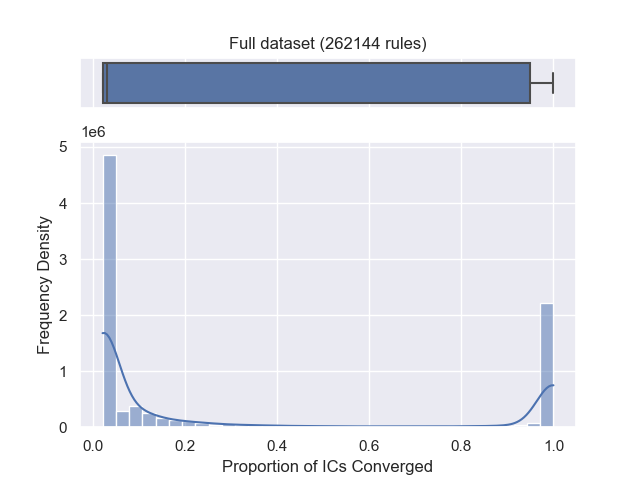
\includegraphics[width=.5\textwidth]{images/full-taxonomy.png}}\hfill
            \subfloat{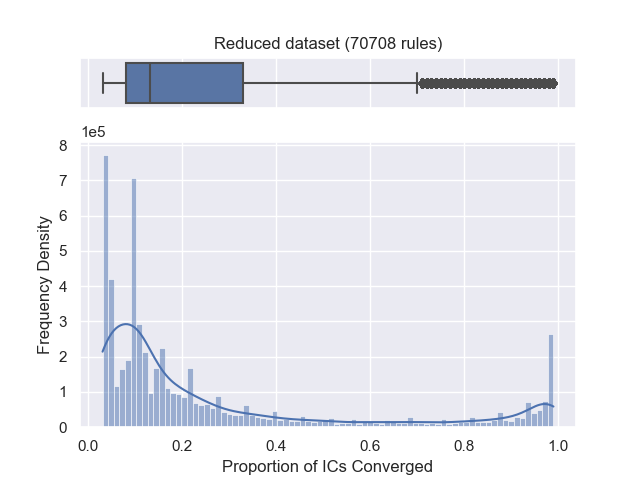
\includegraphics[width=.5\textwidth]{images/reduced-taxonomy.png}}\hfill
            \caption{Distributions of convergence of full and reduced set of life-like CAs}
\label{fig:taxonomy-dist}
\end{figure}

First we consider the two extremities. 23.2\% of rules converge for all initial conditions and 49.8\% of rules converge for only 2 out 100 initial conditions. Note this is the minimum convergence number in our setting since all rules will converge for the trivial initial conditions with density 0 and density 1.  This leaves 27.0\% or 70708 of the original rules remaining. While the original dataset had a median of 3\% convergence, the reduced set of rules present a more even spread with a median of 13\%.

\section{Maze Generation}

We begin by evaluating the effectiveness of the maze generator at maximizing the two fitness metrics. These are the length of the solution path ($p$) and the number of dead ends ($d$). From spot checks on a few examples in the simulator, we find that these two metrics happen to have similar ranges (around 70-100). For this reason we begin by treating them with equal weighting during hyperparameter tuning.\\

\subsection{Hyperparameter Tuning}

We perform a grid search on training hyperparameters across the following ranges
\begin{center}
    \begin{tabular}{ l c }
        \bf Hyperparameter & \bf Values Tried\\
        Number of Epochs & 10, 50, 100\\
        Population Size & 20, 50, 100\\
        Elitism Rate & 0.1, 0.2, 0.5\\
        Mutation Rate & 0.01, 0.05, 0.1
    \end{tabular}
\end{center}

\begin{figure}[!h]
\centering
            \subfloat[Fitness across both metrics, $d$ against $p$.]{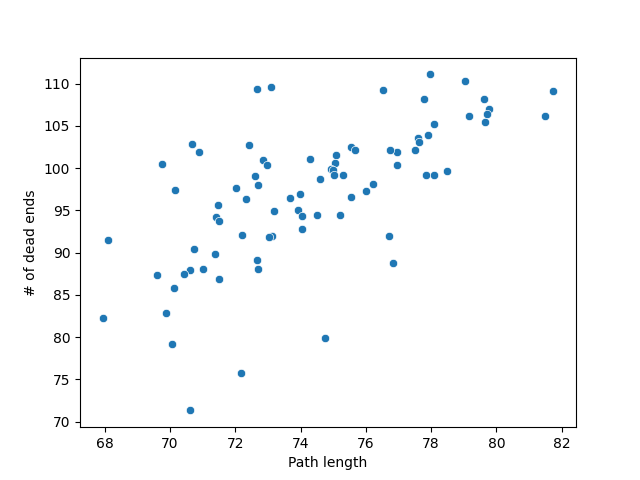
\includegraphics[width=.45\textwidth]{images/maze_hyperparam_notime.png}}\hfill
            \subfloat[Runtime adjusted fitness. $\frac{d}{t}$ against $\frac{p}{t}$ with log axes.]{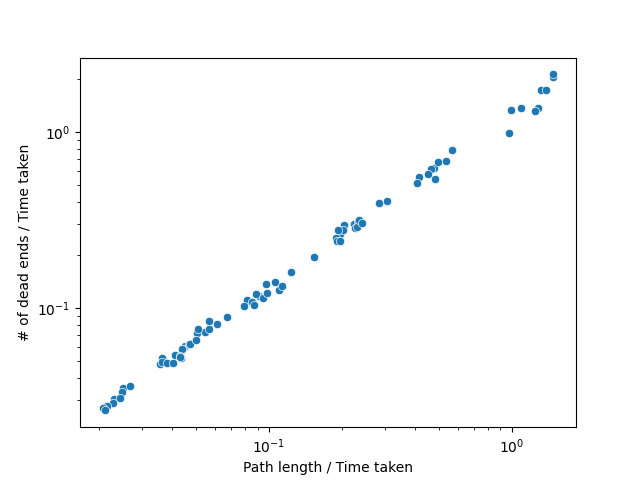
\includegraphics[width=.45\textwidth]{images/log_maze_hyperparam.png}}\hfill
            \caption{Fitness of different hyperparameter configurations across both metrics for maze generation}
\label{fig:maze-hyperparam}
\end{figure}

The optimum metrics achieved are ($d=109.1$, $p=81.8$) with configurations (number of epochs = $100$, population size = $20$, elitism rate = $0.5$, mutation rate = $0.01$). Under a time adjusted measure, we try to optimize for the value of the metric achieved relative to the execution time. Here, the optimum value is ($d=100.5$, $p=69.8$) for configurations (number of epochs = $100$, population size = $20$, elitism rate = $0.1$, mutation rate = $0.05$). This is not significantly worse than the optimum value achieved when disregarding execution time.

\subsection{Ablation Analysis}
Hyperparameter tuning revealed that the lowest mutation rate produced the best results. This suggests that mutation may not be necessary for maze evolution. To test this hypothesis, we conduct an ablation analysis on the genetic operators used. We run 10 maze generations, each for 100 epochs. We use the optimal runtime-adjusted hyperparameters for efficiency. We then repeat this procedure, each time systematically adding and removing genetic operators from the learning procedure. Figure~\ref{fig:maze-ablation} shows a kernel density estimate plot which visualises the area occupied by the optimal results produced by each of these learning procedures.\\

\begin{figure}[!h]
\centering
            \subfloat[Mutation and no crossover]{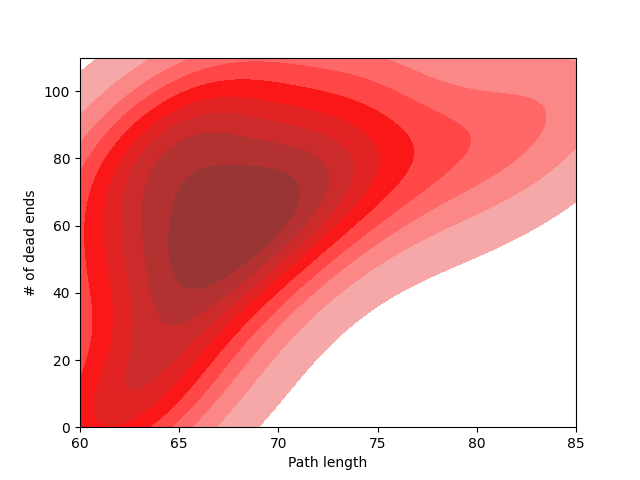
\includegraphics[width=.3\textwidth]{images/maze_eval/cross-kde.png}}\hfill
            \subfloat[Crossover and no mutation]{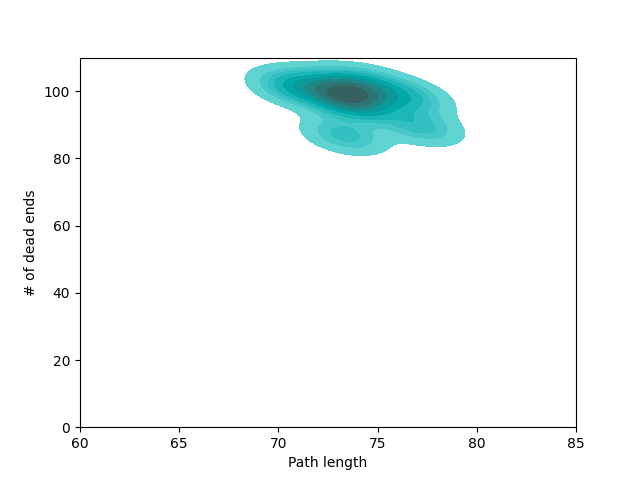
\includegraphics[width=.3\textwidth]{images/maze_eval/mutation-kde.png}}\hfill
            \subfloat[Both mutation and crossover]{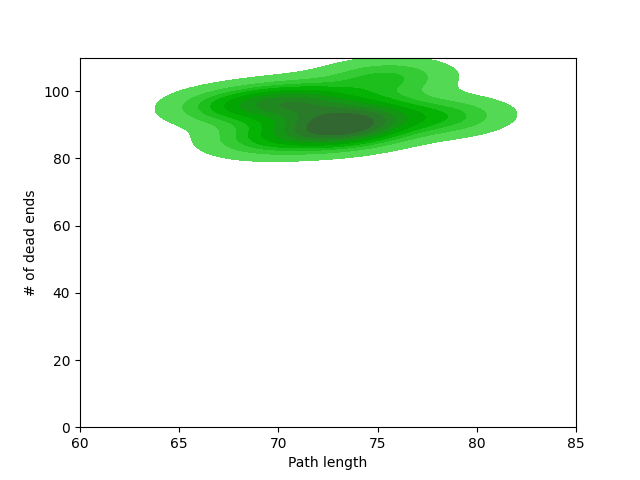
\includegraphics[width=.3\textwidth]{images/maze_eval/both-kde.png}}\hfill
            \caption{Optimum results produced when removing mutation and crossover components for mazes}
\label{fig:maze-ablation}
\end{figure}

It is clear that crossover is important for convergence to a strong solution as the experiment without crossover had a much higher variance in the results produced. However, mutation appears to have a much smaller effect in this case. Without mutation, we obtain a slightly higher variance in results produced and these results tend to have a lower number of dead ends. If both mutation and crossover are omitted, no learning occurs and we find no legitimate mazes in the majority of cases.

\subsection{Objective vs Relative Fitness}

Since we are optimising for two metrics, we can take a linear combination of the objective values of $p$ and $d$ or we can rank each candidate separately by $p$ and $d$ then take a linear combination of the ranks. We call this objective and relative fitness respectively. For each fitness type, we run 20 experiments with a bias of 0.5 (i.e. equal weighting to the two goals) In Figure~\ref{fig:objective} KDE plots show the difference in performance of roulette and truncation selection using each of objective and relative fitness for selection. Note that the x axis here is still objective fitness as that is what the algorithm as a whole is attempting to maximise.\\

\begin{figure}[!h]
\centering
            \subfloat[Objective Fitness]{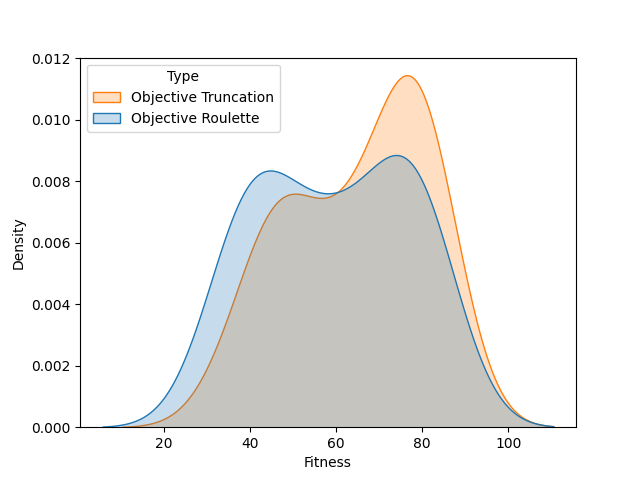
\includegraphics[width=.5\textwidth]{images/objective-fitness.png}}\hfill
            \subfloat[Relative Fitness]{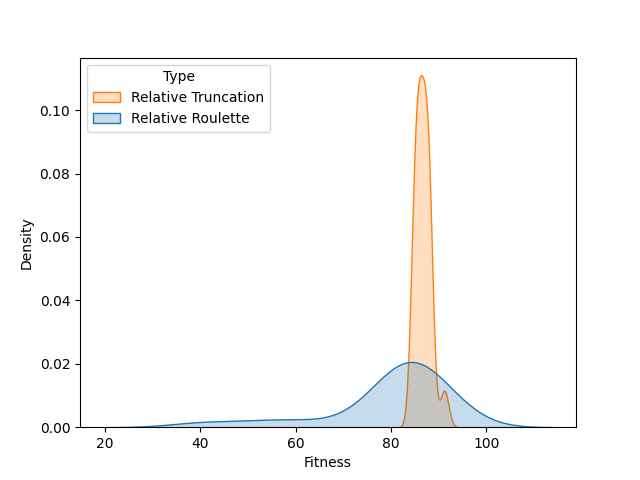
\includegraphics[width=.5\textwidth]{images/relative-fitness.png}}\hfill
            \caption{Objective and relative fitness for roulette and truncation selection}
\label{fig:objective}
\end{figure}

Under both objective and relative fitness, truncation selection outperforms roulette selection on average. There is also a lower variance in the fitness of solutions produced using truncation selection. This is especially exemplified in the case with relative fitness. One reason for this is the decreasing variability in fitness of elite candidates as the population evolves. This makes a roulette selection increasingly likely to pick suboptimal parents. Truncation selection, on the other hand, asserts that a selected candidate will never have a lower fitness than a candidate that has not been selected. However, this can also increase the likelihood of premature convergence since genes within incrementally worse solutions that have potential to produce global optima are lost. Based on the results shown, we opt for a truncation selection using relative fitness. It is interesting to see that a alternative selection criterion, relative fitness, can optimize the objective function better than using the objective function itself for selection.

\subsection{Bias Tuning}
The bias parameter $\lambda$ decides the weighting given to solution path length over number of dead ends when calculating fitness. Although this can be set by the user based on personal preference, we can tune the bias to find the value that maximizes overall fitness  $f(\lambda) = \lambda \hat{p}_\lambda + (1-\lambda)\hat{d}_\lambda$ where $ \hat{p}_\lambda$ and $\hat{d}_\lambda$ are the optimal values discovered by the algorithm under a bias of $\lambda$.\\ 
\begin{figure}[!h]
\centering
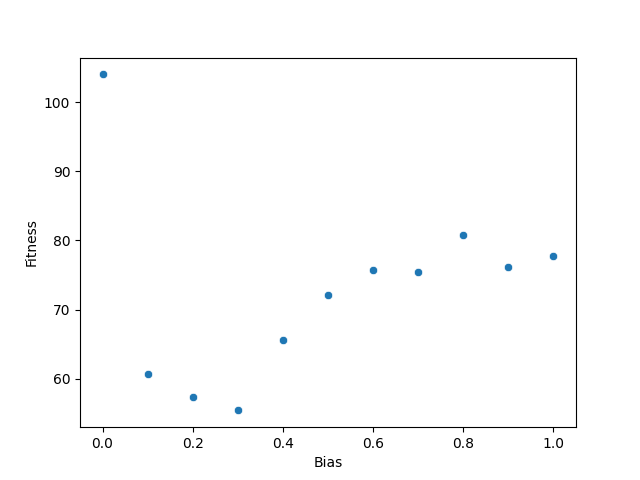
\includegraphics[width=0.7\textwidth]{images/bias-tuning.png}
\caption{Best fitness rule strings discovered under different bias values $\lambda$}
\label{fig:bias-tuning}
\end{figure}
Figure~\ref{fig:bias-tuning} shows that the algorithm performs best for higher bias values except $\lambda=0.0$ which has a very high performance. For a maze with a mix of dead ends and long solution path, the user may find better results from a bias of around 0.5 than around 0.3. Figure~\ref{fig:bias-mazes} shows the top mazes produced for different bias values. Qualitatively these appear to optimize the metrics they are being tested against.\\
\begin{figure}[!h]
\centering
            \subfloat[B16/S1235 ($\lambda=0.0$)]{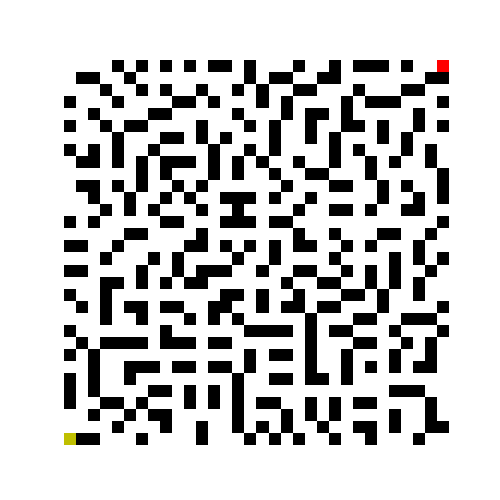
\includegraphics[width=.33\textwidth]{images/0-bias-maze.png}}\hfill
            \subfloat[B2678/S12348 ($\lambda=0.4$)]{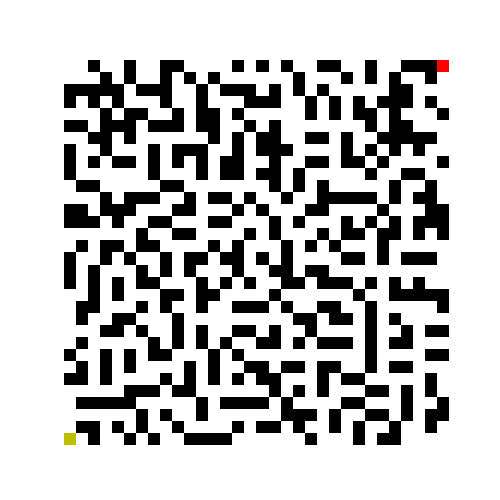
\includegraphics[width=.33\textwidth]{images/40-bias-maze.png}}\hfill
            \subfloat[B238/S12356 ($\lambda = 1.0$)]{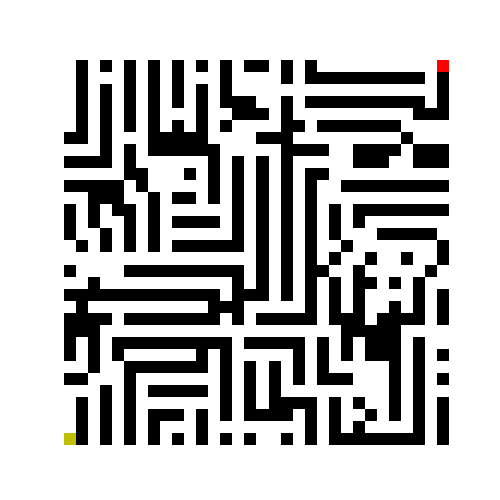
\includegraphics[width=.33\textwidth]{images/100-bias-maze.png}}\hfill
            \caption{Best mazes produced from rules discovered using different bias values}
\label{fig:bias-mazes}
\end{figure}

\section{Life-Like CA}

\subsection{Single Case Evaluation} \label{sub:single-case}

We begin by attempting to learn for a few specific rules to test the efficacy of the learning process. Consider Conway's Life rule B3/S23. In binary this is '000100000001100000' and as an integer it is 16480. Based on spot checks, we use the following hyperparameters\\ 
\begin{center}
    \begin{tabular}{ l c }
        Number of Epochs & 30\\
        Population Size & 20\\
        Number of Initial Conditions & 20\\
        Elitism Rate & 0.2\\
        Mutation Rate & 0.05\\
        Evaluation Steps & 10\\
        Minimum Step Size & 1\\
        Maximum Step Size & 5\\
    \end{tabular}
\end{center}
These have been obtained by looking at common parameters used in the literature\todo{cite}, using parameters from the maze generation experiments, and running spot checks on a few examples. A more rigorous hyperparameter tuning of the final 3 parameters is covered in Subsection~\ref{sub:stepsize}. We test on initial conditions sampled uniformly on density.\\ 

\begin{figure}[!h]
\centering
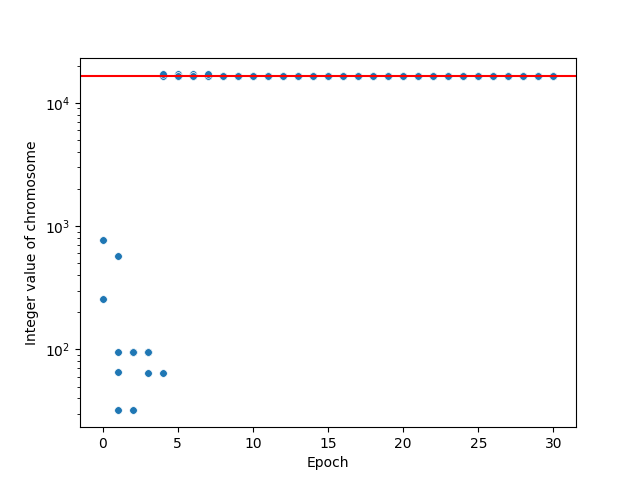
\includegraphics[width=0.7\textwidth]{images/life_like_eval/life-convgraph.png}
\caption{Top 4 elite rules from each epoch in an experiment learning Life. The red line represents the goal.}
\label{fig:life-convgraph}
\end{figure}

Figure~\ref{fig:life-convgraph} shows the algorithm to be very successful at learning the Life rule. In this experiment, the algorithm converges to the correct solution in 5 epochs. At many epochs, and especially after the true rule has been discovered, we see less than 4 points because a few of the elite rules are the same. Note that the graph has a log y-axis, so convergence is extremely fast.\\

\begin{figure}[!h]
\centering
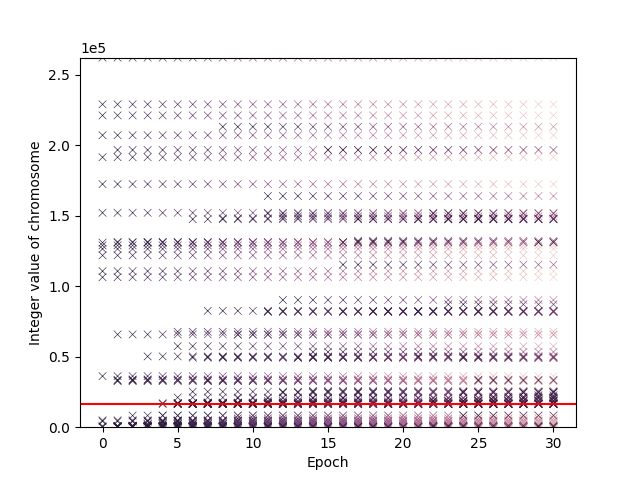
\includegraphics[width=0.7\textwidth]{images/life_like_eval/life-searchgraph.png}
\caption{All visited rules during evolution. Each rule is represented as a dark cross when first discovered and gradually fades in colour from left-to-right. The red line represents the goal.}
\label{fig:life-searchgraph}
\end{figure}

Figure~\ref{fig:life-searchgraph} shows the portion of the search space visited by the algorithm. As we can see, the top areas far from the goal quickly fade away as selection pressure removes such solutions and offspring in this area are no longer produced. We can also see some other dark bands existing far from the goal at epoch 30. The evolution history shows that by epoch 8, all the elite candidates are identical copies of the goal. This means that the dark bands seen at the end of the graph are not local optima but rather instances of the limited types of offspring that can be produced by applying crossover between two identical rule strings representing the goal solution.

\subsection{Ablation Analysis}
Ablation analysis reveals that both mutation and crossover are critical to achieving a performance like this. Consider Figure~\ref{fig:life-ablation}. 'Visited' indicates the number of unique candidates considered by the algorithm in 30 epochs. Under no mutation and no crossover, we see that the population does not evolve at all. The number of visited candidates is equal to the initial population size, 20. With mutation but no crossover, the algorithm is incapable of convergence as it is unable to retain generational knowledge. With crossover but no mutation, the algorithm quickly converges to a local minimum from which it is powerless to escape. This also stagnates the number of candidates visited to 37. When both mutation and crossover are maintained, the algorithm successfully converges to the global minimum.\\ 

\begin{figure}[!h]
\centering
            \subfloat[No mutation and no crossover (visited = 20)]{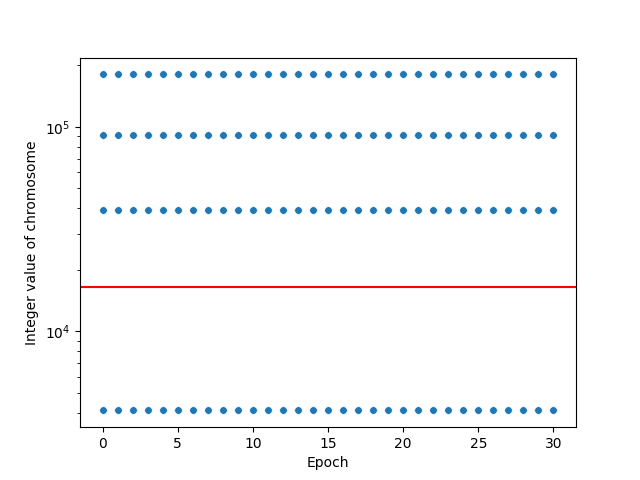
\includegraphics[width=.5\textwidth]{images/life_like_eval/life-nothing.png}}\hfill
            \subfloat[Mutation and no crossover (visited = 90)]{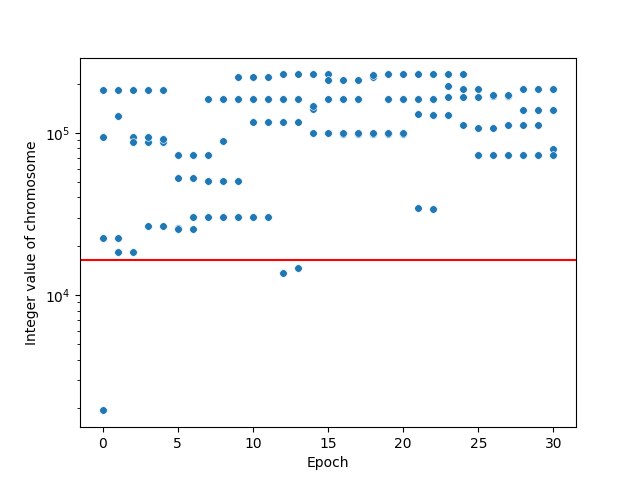
\includegraphics[width=.5\textwidth]{images/life_like_eval/life-no-crossover.png}}\hfill
            \newline
            \subfloat[Crossover and no mutation (visited = 37)]{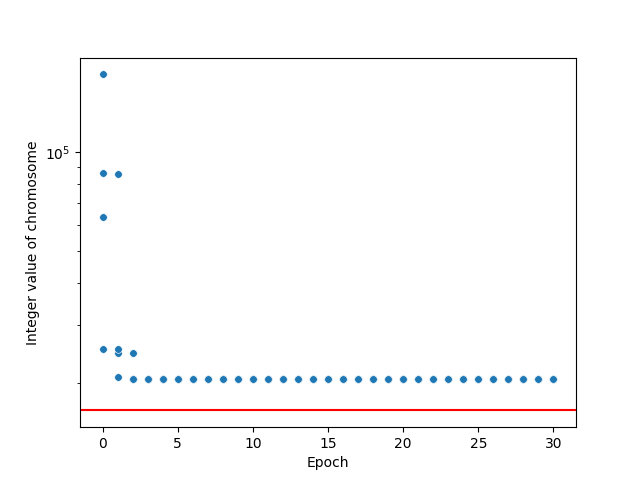
\includegraphics[width=.5\textwidth]{images/life_like_eval/life-no-mutation.png}}\hfill
            \subfloat[Both mutation and crossover (visited = 197)]{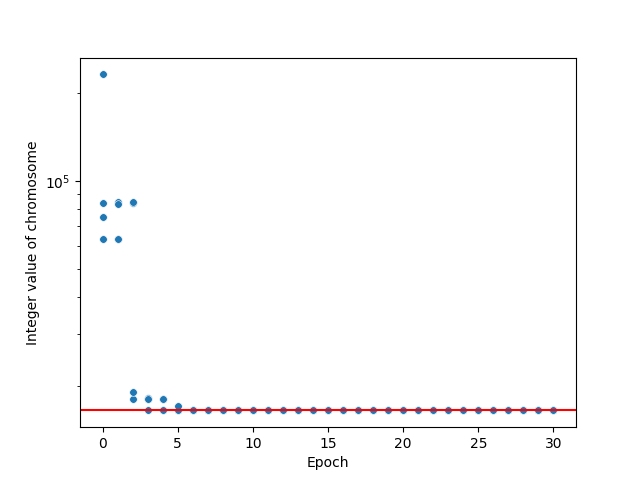
\includegraphics[width=.5\textwidth]{images/life_like_eval/life-both.png}}\hfill
            \caption{Optimum results produced when removing mutation and crossover components for modelling life-like CA}
\label{fig:life-ablation}
\end{figure}

\subsection{Stepsize Tuning}\label{sub:hyperparameter-tuning}
 
Since the rule space is of order $10^6$, performing hyperparameter tuning across all parameters on a representative sample of the search space would be infeasible in the given time frame with the resources available. We find the parameters established in \ref{sub:single-case} to be appropriate based on spot checks on a set of rules covering all 4 Wolfram classes. These bear some similarity to the hyperparameters established in the procedural generation case. One point of interest is optimising the number of evaluations and the stepsize as these factors have considerable effect on the training time.\\

Considering a random uniform stepsize, $\delta_k \sim \mathit{Uniform}(D_{max}, D_{min})$ we set $D_{min} = 1$ since we would like to give the algorithm a chance of learning on very small steps. To determine $D_{max}$, the algorithm is run on 100 goal rules sampled uniformly across the integer rule values and each the loss of each rule is calculated by simulating on 20 random initial conditions. Note that by initialising the population uniformly on rule densities but sampling the goals uniformly on integer values, we ensure that we are not testing giving ourselves an unfair advantage by testing on a subset of the search space where our algorithm is naturally more likely to place initial guesses.\\

\begin{table}
    \centering\hfill
    \subfloat[Average convergence rate]{
        \begin{tabular}{|c||c|c|c|}
            \hline
            $D_{max}$ & \multicolumn{3}{|c|}{Number of Steps } \\
            \hline
            & 1 & 5 & 10 \\
            \hline
            1 & 100\% & 76\% & 52\% \\
            5 & 100\% & 100\%& 100\% \\
            10 & 100\% & 100\%& 100\% \\
            \hline
    \end{tabular}}\hfill
    \subfloat[Average convergence time (epochs)]{
        \begin{tabular}{|c||c|c|c|}
            \hline
            $D_{max}$ & \multicolumn{3}{|c|}{Number of Steps} \\
            \hline
            & 1 & 5 & 10 \\
            \hline
            1 & 9 & 12 & 11 \\
            5 & 9 & 9 & 10\\
            10 & 9 & 9 & 9\\
            \hline
    \end{tabular}}\hfill
\end{table}

Almost all configurations of step number and step size were able to converge to 100\% of the target rules within 30 epochs. The two configurations that failed to do this involved a maximum step size of 1 and many evaluation steps. In the extreme case of the configuration with 10 consecutive steps, only 52\% of targets were learnt successfully. Here, the CA is in the early stages of simulation with many transient patterns, so additional observations appears to be counter-productive. However, we also see that the genetic algorithm can perform surprisingly well calculating fitness on a single immediate observation of the goal rule after 1 time step. Computationally, this is very efficient compared to multiple stochastically chosen observations over longer periods of time. \\

There is some variability in the average convergence times obtained when repeating this experiment so we only consider average convergence time to the nearest epoch. Almost all configurations seem equally good in this regard with the exception of configurations with very small step sizes or very high number of observations. In general, many late-stage observations can dilute information gathered in the early-stages of observation. With the top configurations tested, these algorithms are able to find the correct solution after considering less than 130 candidates. This is extremely impressive given that this "visited region" makes up less than $0.05\%$ of the entire search space.\\

However, it is also important to note the size of the test set. The set of 100 targets, despite being representative of the all possible rule strings, also makes up less than $0.05\%$ of the entire search space. It is plausible to imagine that there is a section of the search space in which our algorithm performs badly but has not been represented in the small test set. With additional time and computational resources, it would be sensible to run this experiment again with a larger test set to see if any rules emerge that cannot be learnt by the algorithm in 30 epochs.

\subsection{Fitness Functions}

We now perform the same hyperparameter grid search on the second fitness function designed: multi-resolution loss. This function takes 3 differently sized smoothing convolutions of the true and surrogate CA, XORs them with each other to get the difference in density in a region around each cell, and takes the average of these differences. The reasoning behind this method is that we expect candidates with similar genotypes to have similar phenotypic behaviour. Therefore, we would expect similar rules to create patterns of similar density in different regions of the lattice. A convolution leverages this effect since the loss between two states with a slight phase shift would be much higher using single-resolution loss than using multi-resolution loss.\\

\begin{table}
    \centering\hfill
    \subfloat[Average convergence rate]{
        \begin{tabular}{|c||c|c|c|}
            \hline
            $D_{max}$ & \multicolumn{3}{|c|}{Number of Steps } \\
            \hline
            & 1 & 5 & 10 \\
            \hline
            1 & 96\% & 63\% & 52\% \\
            5 & 96\% & 97\%& 98\% \\
            10 & 96\% & 98\%& 98\% \\
            \hline
    \end{tabular}}\hfill
    \subfloat[Average convergence time (epochs)]{
        \begin{tabular}{|c||c|c|c|}
            \hline  
            $D_{max}$ & \multicolumn{3}{|c|}{Number of Steps} \\
            \hline
            & 1 & 5 & 10 \\
            \hline
            1 & 11 & 12 & 15 \\
            5 & 12 & 12 & 12\\
            10 & 10 & 11 & 12\\
            \hline
    \end{tabular}}\hfill
\end{table}

We find that multi-resolution loss is patently worse than single resolution loss. When learning with multi-resolution loss, all configurations are able to learn fewer targets and convergence time is higher. This suggests that the algorithm is not using high level, stable features to distinguish between different CAs. Instead, it is using high-fidelity behaviour in the early chaotic stages of each CA to uniquely identify them. This also explains why performance decreases as the number of observations increase.

\subsection{Class Evaluation}
\todo{Class evaluation}

\section{Gray-Scott Models}

The search space for Gray-Scott models is infinite so in the style of Giampaolo et al.\cite{giampaolo2022physics}, we consider four example targets.

\begin{center}
    \begin{tabular}{ |l|c|c| }
        \hline
        Target Name & Feed Rate ($f$) & Kill Rate ($k$)\\
        \hline
        Flower & 0.055 & 0.062\\
        Zebrafish & 0.035 & 0.060\\
        Soliton & 0.030 & 0.060\\
        Mitosis & 0.028 & 0.062\\
        \hline
    \end{tabular}
\end{center}

We choose to train a population of 25 candidates for 30 epochs since similar values worked effectively for life-like CA and limited computational resources mean that it is infeasible to run the range of experiments required on larger populations or for longer periods. We use a linear truncation loss, splatter initialisation for each CA, and random uniform initialisation of the parameters in the ranges ($0.0 \leq f \leq 0.30$) and ($0.0 \leq k \leq 0.08$).

\subsection{Evolutionary Strategy}

Using a self-adapting evolutionary strategy, we find that the patterns converge to local optima. Consider the flower pattern. Figure~\ref{fig:flower-fail} shows both the state and control parameters converging at around 17 epochs. However, the converged solution of ($f = 0.138, k = 0.036$) is not the true solution.\\

\begin{figure}[!h]
\centering
            \subfloat[State paramaters]{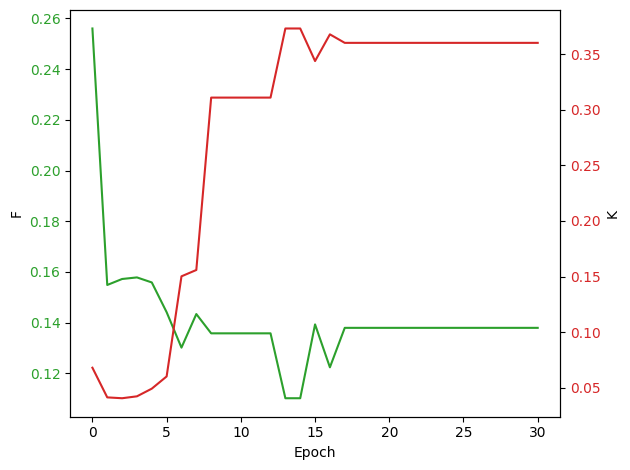
\includegraphics[width=.5\textwidth]{images/flower-params.png}}\hfill
            \subfloat[Control parameters]{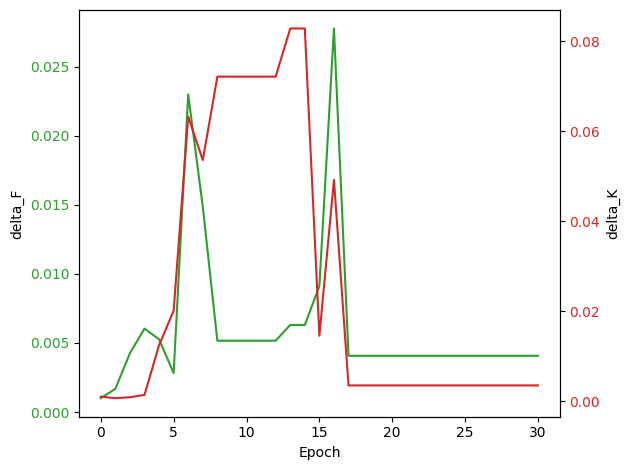
\includegraphics[width=.5\textwidth]{images/flower-derivs.png}}\hfill
            \caption{Evolution of \textit{flower} pattern using evolutionary strategy (population size = 20)}
\label{fig:flower-fail}
\end{figure}

Increasing the population size does not appear to resolve matters. Changing the discrete Laplacian operator to the alternative presented by Compeau\cite{compeau}
\[
  K= \begin{bmatrix}
    0.05 & 0.2 & 0.05\\
    0.2 & -1 & 0.2\\
    0.05 & 0.2 & 0.05
  \end{bmatrix}
\]
also appears to have no effect. These are shown in Figure~\ref{fig:more-fails}

\begin{figure}[!h]
\centering
            \subfloat[State paramaters for \textit{zebrafish} pattern (pop size = 50, Laplacian = nine-point stencil)]{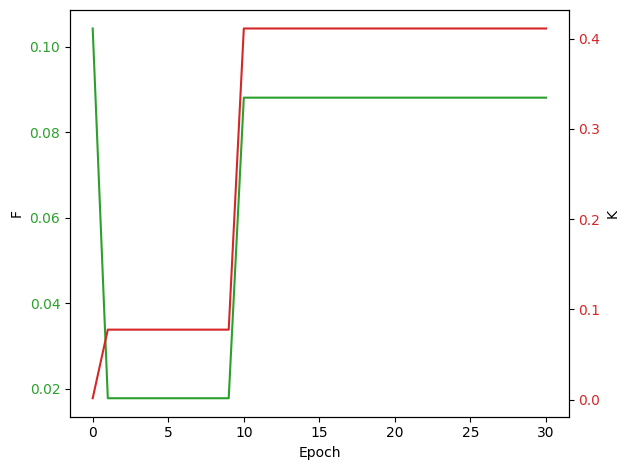
\includegraphics[width=.5\textwidth]{images/zebra-params.png}}\hfill
            \subfloat[State paramaters for \textit{soliton} pattern (population size = 25, Laplacian = Compeau operator)]{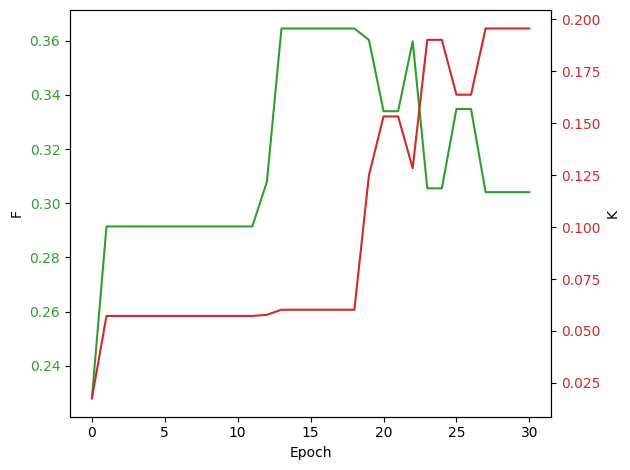
\includegraphics[width=.5\textwidth]{images/soliton-params.png}}\hfill
            \caption{Evolution of Gray-Scott models with different population sizes and Laplacian operators}
\label{fig:more-fails}
\end{figure}

\subsection{Genetic Algorithm}




\todo{Test GA}
\todo{Add image of goal vs pred}


\bibliographystyle{unsrtnat}
\bibliography{bibs/bib}

\end{document}